\documentclass[twoside,a4paper]{report}
\usepackage[T1]{fontenc}
\usepackage[utf8]{inputenc}
\usepackage[english]{babel}
\usepackage{hyperref}
\usepackage[round]{natbib}
\usepackage{float}
\usepackage{ amssymb }
\usepackage{array, makecell}
\usepackage{booktabs, tabularx}
\newcolumntype{L}{>{\raggedright\arraybackslash}X}
\usepackage{setspace}
\usepackage{graphicx}
\usepackage{csvsimple}
\usepackage{mathtools}
\usepackage{titling}
\usepackage{eqnarray, amsmath}
\usepackage{endnotes}
\usepackage{lscape}
\usepackage{verbatim}
\usepackage{pdfpages}
\usepackage[toc,page]{appendix}
\usepackage{tikz}
\usetikzlibrary{shapes,arrows}
\usepackage[labelfont=bf]{caption}
\usepackage{subcaption}
\DeclareMathOperator*{\argmin}{arg\,min}
\DeclareMathOperator*{\argmax}{arg\,max}
\newcolumntype{L}{>{\centering\arraybackslash}m{1.6cm}}
\usepackage[hmarginratio=1:1]{geometry}
\graphicspath{ {./images/} }
\newcommand{\subtitle}[1]{%
	\posttitle{%
		\par\end{center}
	\begin{center}\LARGE#1\end{center}
	\vskip0.5em}%
}

\title{ALBERT LUDWIGS UNIVERISTY OF FREIBURG
\\{\Large MASTER THESIS}}

\subtitle{\line(1,0){250}\\\textbf{\Huge Multisite RNA-RNA Interaction Prediction}\\\line(1,0){250}}	

\author{Yogapriya Ayyanarmoorthy}
\date{\today}



\begin{document}
	
	\maketitle
	
	\tableofcontents
	
	\chapter{Introduction}
	RNA molecules play important roles in various biological processes.Their regulation and function are mediated by interacting with other molecules. 	Forming base pairs between two RNAs, called RNA-RNA interactions (RRI). There are fast and reliable single interaction site (S-RRI) prediction tools like IntaRNA, that often show the additional sites within their suboptimal list, ie. are capable of modelling all sites individually but not in a joint prediction. Many RNAs interact via multiple synchronous, non-overlapping subinteractions (M-RRI), e.g. OxyS-fhlA. The simultaneous prediction of both intra- and inter-molecular base pairing allowing for multiple sites is computationally expensive. Some known approaches are IRIS, piRNA, NUPACK. Here we use a S-RRI prediction tool (namely IntaRNA) for the prediction of M-RRI.
	
	\section{Biological Background of RNA}
	In this thesis, I will focus on Ribonucleic acids (RNA). First of all, I would like to provide the basic biological background that is essential for the thesis. Ribonucleic acid, or RNA is one of the three major biological macromolecules that are important for all known forms of life (along with DNA (deoxyribonucleic acid) and proteins). The "central dogma" of molecular biology states that the flow of genetic information in a cell is from DNA through RNA to proteins: “DNA makes RNA makes protein” (as first suggested by Jean Brachet in 1960 )\citep{brachet1956remarks}. The process by which DNA is copied to RNA is called \textit{transcription}, and that by which RNA is used to produce proteins is called \textit{translation}. RNAs also play an important role in protein synthesis. \\
	
	 DNA is double stranded and RNA is a single-stranded molecule. Each strand of RNA is a sequence of four building blocks called \textit{nucleotides}. Each nucleotide contains Sugar, phosphate and nitrogen containing bases. The sugar and phosphate groups form the backbone of RNA strand and the bases bond to each other.The RNA molecules are represented as a sequence $S \in \{A, C, G, U\} ^*$, where A (adenine), C (cytosine), G (guanine), U (uracil) are the bases of the nucleotide chain.\\
	 
	According to their potential for coding, RNA's are classified into two major categories i.e., coding RNAs and noncoding RNAs. Coding RNAs mostly refers to mRNA that encodes protein to act as different components including cell structures, signal transductors and enzymes. Noncoding RNAs act as cellular regulators with no protein encoding.\\
	Complementary bases $C$-$G$ and $A$-$U$ form stable base pairs with each other using hydrogen bonds. These are called Watson-Crick pairs. Also important are the weaker $U$-$G$ wobble pairs. Together they are called \textit{canonical base pairs}. In general, Isolated base pairs are unstable. If two interacting bases belonging to the same molecule of RNA form \textit{intra-molecular} structures and if they belong to different molecules of RNA form \textit{inter-molecular} structures, as seen in figure ~\ref{fig:secondarystructure}\\
	
	The prediction of RNA-RNA interaction is intended to predict these intermolecular structures between two RNA molecules, an extremely important step in understanding the role of ncRNAs. However, Intra and intermolecular structures are not mutually exclusive.\\
	
	\begin{figure}[h]
	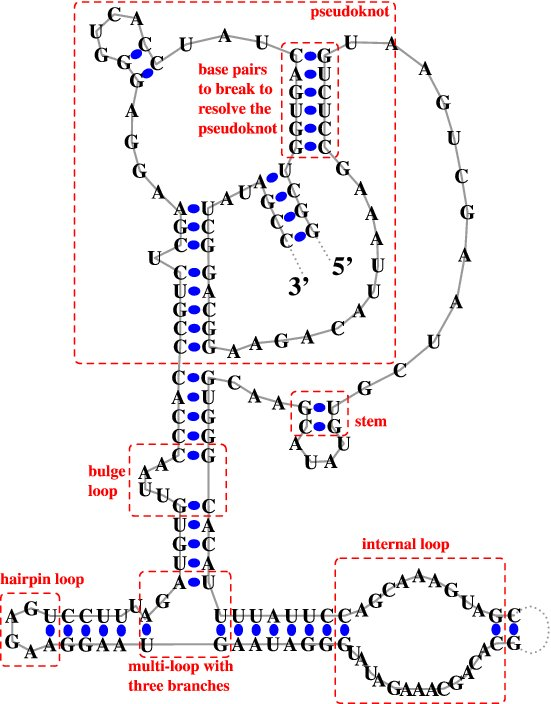
\includegraphics[width=0.7\linewidth]{secondary_structure}
	\centering
	\caption{Schematic representation of the secondary structure (a set of base pairs) for the RNase P RNA molecule of Methanococcus marapaludis from the RNase P Database. Thick blue dots represents base pairs and red dashed boxes represent structural features such as stacking, bulges, hairpin , interior, multi loops and pseduoknot structure. This Figure was taken from the RNAStrand webpage.
	\label{fig:secondarystructure} 
    \citep{andronescu2008rna}}
	\end{figure}

	Single stranded nucleic acid sequences contain many complementary regions that can form double helices when the molecule is folded back onto itself. The resulting pattern of double helical stretches interspersed with loops is called the \textit{Secondary} structure of an RNA.\\
	\section{Formal background of RNA}
	Here in this section, I would like to bring up the formal definitions of ribonucleic acid.
	\subsection{RNA Structure}
	Formally, an RNA secondary structure $P$ of $S$ is a set of base pairs:\\
	\begin{center}
	 $ P \subseteq \{(i, j) | 1 \leq i < j \leq n $, $ Si $ and $Sj$ complementary \},\\
	\end{center}
	where $ n = |S| $ and for all $(i, j) , ( i', j' ) \in  P:$\\
	\begin{center}
	$(i = i' \Leftrightarrow j = j')$ and $ i \neq j'$ \\
	\end{center}

	They are different types of RNA secondary structures they are nested
	and crossing structures. Crossing structures contain pseudo-knots, where two structure parts overlap. Nested structures doesn't have any crossing arcs.\\

	To form a valid secondary structure, the base pairs must satisfy a number of limitations. Let the bases be numbered from 1 to n in a sequence. If the bases are complementary, a base pair may form between positions $i$ and $j$ , and if $|j - i | \geq 4$, since there must usually be at least three unpaired bases in a hairpin loop. Let bases $k$ and $l$ form another allowed pair. The pair $k - l$ is said to be compatible with the pair $i - j$ if the two pairs can be present in a structure simultaneously. Pairs are compatible if they are non-overlapping (e.g. $i<j<k<l$ ) or if one is nested within the other (e.g. $i<k<l<j$ ). The Final case, where the pairs are interlocking (e.g. $i<k<j<l$ ) is called  pseudo-knot.These pairs are assumed to be incompatible with
	most dynamic programs. An allowed secondary structure is a set of base pairs that are all compatible with each other.\\
	
	\subsection{Nested secondary structure}
	Nested secondary structures can be uniquely decomposed into so called loops or secondary structure elements. Depending on the number of enclosed base pairs (BP) and unpaired bases (UB), different types of secondary structure elements are distinguished.They are hairpin loop, stacking, bulge loop, internal loop, multi loop. \\
	Let $S$ be a fixed sequence. Further, let $P$ be an RNA structure for $S$.
	\begin{itemize}
		\item a base pair $( i, j ) \in P$ is a \textit{hairpin} loop if\\
			$	\forall i < i' \leq j' < j : (i', j') \notin P. $

		\item a base pair $( i, j ) \in P$ is a \textit{stacking} if\\
		$(i + 1 , j - 1 ) \in P $
		\item two base pairs $ (i, j) \in P$ and $(i' ,j' ) \in P$ form  an \textit{internal} loop $(i,j,i',j')$ if \\
		$i < i' < j' < j $ ; $ (i' - i)+( j - j') > 2$ ; no base pair $(k,l)$ between $(i, j)$ and $(i',j')$
		\item An internal loop is called left (right, resp.) \textit{bulge} if\\
		$ j = j' +1 $ or $ i' = i+1$
		\item A k-\textit{multiloop} consists of multiple base pairs, $(i_1,j_1)$... $(i_k,j_k) \in P$ with a closing base pair $(j_0, i_{k+1}) \in P$ with the property that \\
		$\forall 0 \leq l \leq k : ( j_l < i_{l'+1})$ ; $\forall 0 \leq l , l' \leq k$ is true that there is no base pair $(i' ,j') \in P$ with $i' \in [j_l...i_{l+1}]$ and $j' \in [j'_l...i_{l'+1}]$ .
		\item $(i_1,j_1)...(i_k, j_k)$ are called the \textit{helices} of the multiloop.\\
 	\end{itemize}
 
 
 	 \citeauthor{DeVoe1962TheSO} discovered that vertical stacking of bases gives largest contribution to the stability of the RNA helix. The stacking of unpaired bases is less predictable and stable than the paired bases. Hence, the directly neighboured bases must be taken into account while estimating the energy contribution of a  base pair, that results in the \textit{Nearest Neighbor Model} \citep{borer1974stability}.\\
 	 
 	 \subsection{Nearest neighbor model and energy contributions }
 	 
 	 The Nearest Neighbor Model enables the calculation of a free energy estimate for a given RNA secondary structure. For the performance of work, the free energy can be taken as the amount of energy stored in a system. The positive energy is in the form of heat  and the negative energy is used to destroy the system. Always, lower the energy gives more stable the system. Hence, for the \textit{most stable structure} of RNA , we go for \textit{minimum free energy (MFE)}. The energy difference between the reference state to the system is measured. We have a reference system which we use to understand the stability of the system. ie., $ E(\phi) =0 $. Hence , we need to check not only the hydrogen bonds but also the stacking stability.The Nearest Neighbor Model uses a loop-based structure decomposition. To avoid the duplication of stacking, only inner stacking are taken into account. \\
 	 
 	 \textit{The terminal mismatch} consists of the first unpaired bases immediately after the stacking. The identity of the terminal mismatch provides the energy of the loop. In Bulge or Internal loop also we have the same energy contribution. Energy contributions for external base pairs, which are not enclosed by any other base pairs, are referred to as textit{dangling end contributions}.\\ 
 	 The energy $E(P)$ ~\ref{eq:1} of a nested secondary structure $P$ can be estimated by the sum of loop contributions (see Figure ~\ref{fig:energycontribution})\\
 	 
 	 \begin{equation}
 	 \label{eq:1}
 	 E(P) = \sum_{(i,j) \in P} \begin{cases}
 	 e^H(i,j) & : \text{if hairpin loop}, \\
 	 e^{SBI}(i,j,k,l) & : \text{if stack/bulge/internal loop} ,\\
 	 e^M(i,j,x,x') & : \text{if Multi loop},
 	 \end{cases}
 	 \end{equation}
 	 
 	 Where $e^H$, $e^{SBI}$ and $e^M$ tells the context sensitive energy contributions of the loops. Where $(k,l)$ represents the enclosed base pair of stack,bulge or internal and $x$ represents the unpaired bases and $x'$ represents the helices enclosed in the multi loop. We can see that there is an exponential number of possible multi loop composition. The energy for them can be calculated as below \\
 	 \begin{center}
 	 $e^M(i,j,x,x')= e^M_a+e^M_bx+e^M_cx'$\\
 	\end{center}
 	 where the pseudo energy parameter $e^M_a$ scores the multi loop closing base pair $(i,j)$ , $e^M_b$ represents the penalty for directly enclosed unpaired bases $x$ and $e^M_c$ represents the number of enclosed helices $x'$.
 	 Thus the nearest neighbor model gives the energy contributions for the loop types. \\
 	 
 	 \begin{figure}[h]
 	 	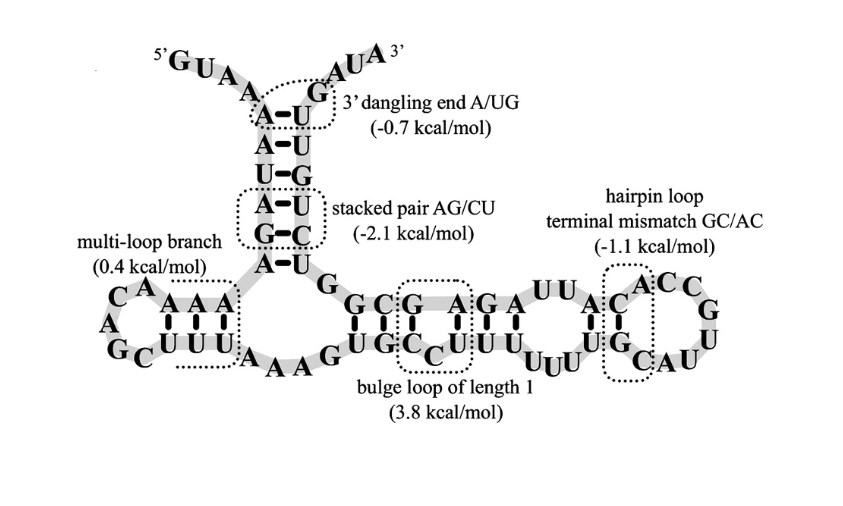
\includegraphics[width=0.9\linewidth]{energy}
 	 	\centering
 	 	\caption{Energy contributions of loops. \citep{andronescu2010computational}}
 	 	\label{fig:energycontribution}
 	 \end{figure}
 	 
 	 
 	 From the above energy model, We can define a recursive dynamic programming algorithm to compute the structure which minimizes the energy function,this is called minimum free energy (mfe) structure. This algorithm was introduced by \citep{zuker1981optimal}.\\
 	 
 	 The basic substructures of the secondary structure of the RNA sequence (i.e., stack, hairpin, internal and multi loop) are independent of each other and the energy of the secondary structure is assumed to be the sum of the energies of the substructure. The algorithm is executed in two steps with a single RNA sequence as input. Firstly, the minimum free energy of the input RNA sequences has been calculated , then traceback is used to recover the secondary structure with the base pairs. Thus given an RNA sequence $S$, Zuker’s algorithm predicts the non-crossing, minimal energy structure $P$ of $S$ in $O(n^3)$ time and $O(n^2)$ space.\\
 	 
 	 \subsection{Structure probabilities and McCaskill algorithm}
 	 Let's discuss about the structural information in terms of probabilities. According to the principal of maximum entropy \citep{jaynes1957information} the best probability distribution for the calculation of the structure or base pair probability is the \textit{Boltzmann Distribution}. These probabilities are calculated according to the Boltzmann weight. For RNA structures the unit of the energy value is $\frac{kcal}{mol}$ or $\frac{J}{mol}$. The RNA structure energy is been rescaled for boltzmann weight computation. i.e., We replace boltzmann constant $k_B$ with "mol-scaled" gas constant $R$\\
 	 
 	 \begin{center}	 
 	 \[ 
 	 w(P)= exp\left( \frac{-E(P)}{RT} \right)
 	 \]
 	 \end{center}
 	 
 	 Where $E(P)$ represents the state energy , $R $ represents the gas constant and $T$ is the temperature.\\
 	 The partition function $Z$ can be calculated using the Boltzmann weights. $Z$ is the sum of the Boltzmann weights of all states within $P$. \\
 	 \begin{center}	 
 	 	\[ 
 	 	Z= \sum_{P \in \mathcal{P}} w(P)
 	 	\]
 	 \end{center}
 	 
 	 $Z$ is used for the calculation of structure and base pair probabilities. So in the total sum, the distribution does not change from a macroscopic point of view,therefore thermodynamic balance is reached.\\
 	 The probability of an RNA structure $P$ is given by \\  
 	  \begin{center}	 
 	 	\[ 
 	 Pr[P|\mathcal{P}] = \frac{w(P)}{Z} 
 	 	\]
 	 \end{center}
  	 and normalising with the partition function $Z$ for the structure ensemble $\mathcal{P}$.  \\
  	
  	 We can also calculate the probabilities of unpaired regions. Formally, we will identify the probability of the subsequences i..j to be unpaired by $\mathcal{P}_{i,j}^{u}$. This probability depends on  on the whole ensemble of structures that can be formed by the RNA molecule of interest. Thus, it can be computed by\\
     \begin{center}	 
     	\[ 
     	\mathcal{P}_{i,j}^{u} = \frac{Z^u_{i_j}}{Z}
     	\]
     \end{center}
 	 where $Z^u_{i_j}$ is the partition function of all structures where the subsequence i..j is unpaired.\\
 	 
 	 i.e., 
 	 \begin{center}	 
 	 	\[ 
 	 	Z^u_{i_j}= \sum_{P \subset \mathcal{P}_{i,j}^{u}} w(P) = Z(\mathcal{P}_{i,j}^{u})
 	 	\]
 	 \end{center}
  
  	 where $\mathcal{P}_{i,j}^{u}$ is the ensemble of all structures that are unpaired between i and j.\\
  	 
  	  i.e., 
  	 \begin{center}	 
  	 
  	 	$\mathcal{P}^u_{i,j}$= $\{P \mid \nexists (k,l) \in P\ : i \leq k \leq j $ or $ i \leq l \leq j\}\subseteq \mathcal {P}_{all}$,
  	 
  	 \end{center}
  	 
  	 Where $\mathcal {P}_{all}$ is the ensemble of all structures that can be formed from a sequence. The calculation of accessibility of single stranded regions is carried out using  unpaired probability \citep{muckstein2006thermodynamics}, hence it is very important. 
  
 	 The below figure ~\ref{fig:unpaired} was inspired by the lecture material of RNA bioinformatics lecture .\\
 	 
 	 \begin{figure}[tb]
 	 	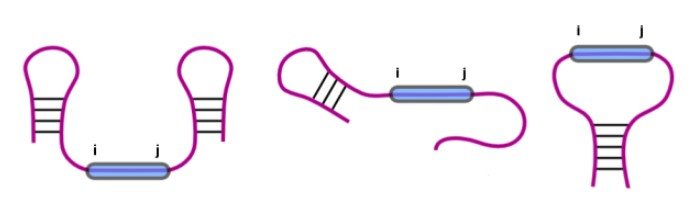
\includegraphics[width=0.8\linewidth]{unpaired}
 	 	\centering
 	 	\caption{Examplary structures that are unpaired in the subsequence i..j.}
 	 	\label{fig:unpaired}
 	 \end{figure}
  
 	 Different probabilities can be calculated using McCaskill algorithm. The McCaskill algorithm \citep{mccaskill1990equilibrium} is used to calculate the partition function $Z$ for a given sequence $S$, which can be used to compute probabilities. It enables efficient computing of the probabilities of the structure of the RNA as well as the probability that a certain base pair is formed. In addition, unpaired probabilities for subsequences can be calculated that reflect the accessibility of RNA parts for other interactions.\\ 
 	
	
	\section{RNA-RNA Interaction}
 	The interaction of RNA molecules is an essential factor for regulatory processes in all organisms. Computational prediction of RNA-RNA interactions (RRI) is a central methodology for the specific investigation of inter-molecular RNA interactions and regulatory effects of non-coding RNAs. RNA–RNA interactions are fast emerging as a major functional component in many newly discovered non-coding RNAs. They are important in many basic cellular activities including transcription, RNA processing, localization, and translation. Interacting RNA strands is classified into two types. ie., Intermolecular and Intramolecular. Many RNA species function is guided by their structure, which is defined by intramolecular base pair formation. Small prokaryotic RNAs display evolutionary unstructured regions that control the expression of their target mRNAs by intermolecular base pairing \citep{wright2013comparative}. Hence, The prediction of both functional intramolecular and intermolecular RNAs are important bioinformatics tasks. \\
 	
 	Let's see about some simple RNA-RNA interactions. In \textit{splicing} , small nuclear RNA's (snRNA) can recognize intronic regions of precursor messenger RNAs(mRNA) which is the important step in identifying the RNA splicing products \citep{modrek2002genomic}. In \textit{translation} transfer RNAs(tRNA) interact with messenger RNAs(mRNA) by reading the three letter code and define amino acid sequence \citep{selmer2006structure}, \citep{ibba2000aminoacyl}. In RNA modification, small nucleolar RNAs(snoRNA) guide the modification of ribosomal RNAs(rRNA) \citep{kiss2002small}. In microRNA (miRNA) targetting, the base pairing between an miRNA and mRNA leads to degradation or translation inhibition of the mRNA \citep{bartel2004micrornas}. For RNA function and regulation these examples gives us the importance of the RNA-RNA interaction. \\
 		
 	In order to allow highly accurate predictions, state-of-the-art methods not only take into account the stability (energy) of possible RNA–RNA interactions, but they also take the accessibility of the interacting subsequences \citep{umu2017comprehensive}.\\
 	
 	\subsection{Formal background of RNA-RNA interactions}
 	Here, we will see the formal background of RNA-RNA interactions.\\
 	In general RNA–RNA interaction prediction (RIP) problem, given two RNA sequences $S^1$ and $S^2$ (e.g., an antisense RNA and its target), the RIP problem asks one to predict their joint secondary structure. A joint secondary structure between $S^1$ and $S^2$ is a set of “pairings” where each nucleotide of $S^1$ and $S^2$ is paired with at most one other nucleotide, either from $S^1$ or $S^2$ \citep{alkan2006rna}.  \\
 	
 	The RNA-RNA interaction is the combination of the set all of all base pairs in $S^1$ , set of all base pairs in $S^2$ and the total intermolecular base pairs between two sequences. Formally, the RRI can be modelled as RRI = $ \uplus $ bp ($S^1$) $ \cup $ $\uplus$ bp ($S^2$) $\cup$ $\uplus$ ($Inter$). Basically, the set of all base pairs of $S^1$ is $P^1$ and $S^2$ is $P^2$ , then $Inter$ is $I$ which denotes the set of all intermolecular base pairs. \\
 	
 		\begin{center}
 		RRI =  $P^1$ $ \cup $  $P^2$ $\cup$ $I$
 		\end{center}
 	
 
	 	\begin{figure}[tb]
		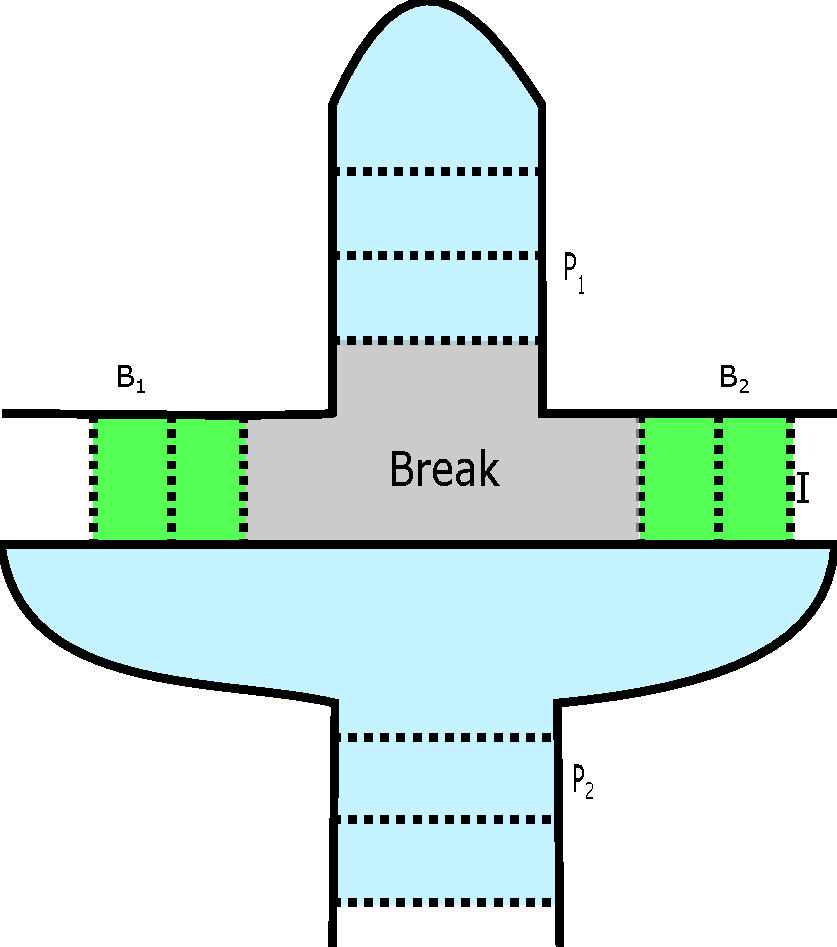
\includegraphics[width=0.6\linewidth]{rnarna.pdf}
		\centering
		\caption{The RNA-RNA Interaction is the union of all base pairs in sequence 1 and sequence 2 are denoted as $P^1$ and $P^2$ respectively. $I$ denotes the union of all intermolecular base pairs. $B_1$, $B_2$ are the interaction blocks. Break is the loop enclosed by two inter-molecular base pairs that also contains positions involved in intra-molecular base pairs}
		\label{fig:rnarna}
	\end{figure}
	
 		\begin{figure}[tb]
 		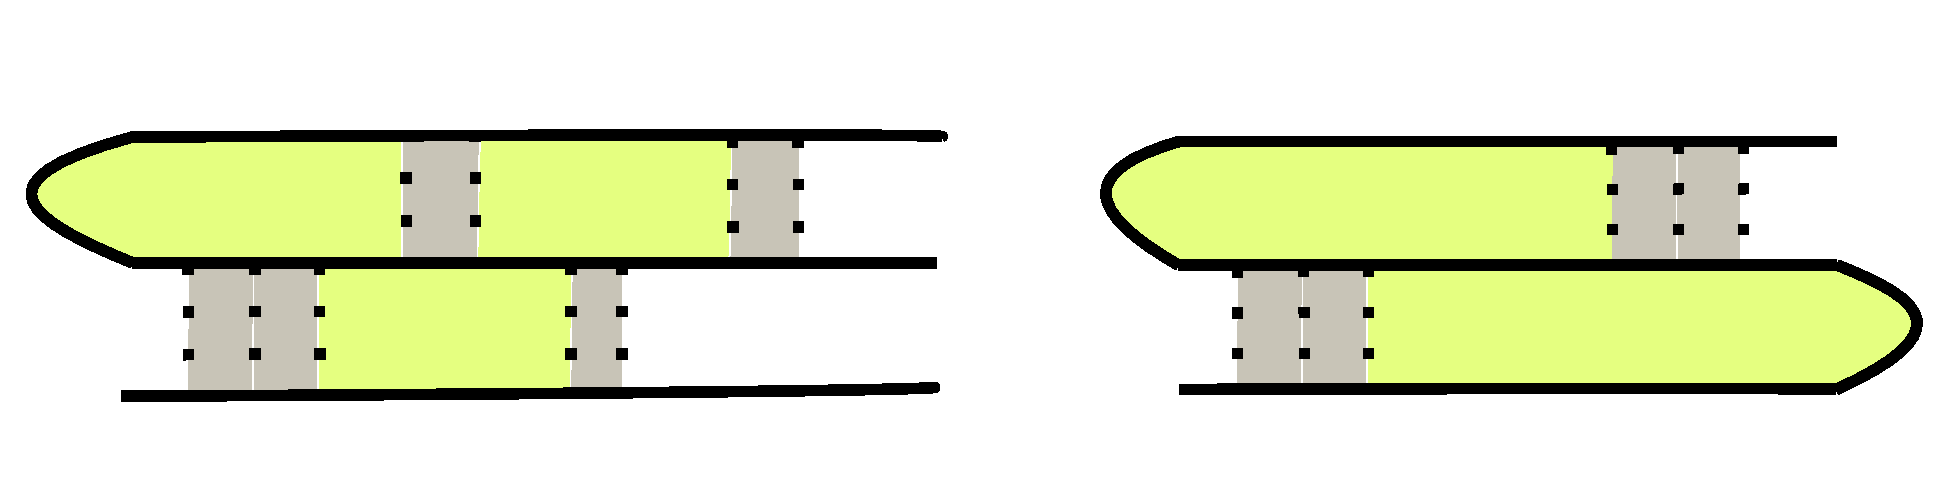
\includegraphics[width=1.0\linewidth]{pseudoknot.pdf}
 		\centering
 		\caption{ The left side figure shows the Positions are not paired within the loop. This problem starts with the pseudoknot which is shown in the right side figure where the same problem exists for the scoring of crossing structures. }
 		\label{fig:pseudoknot}
 	\end{figure}
 	
 	The same problem we have for the scoring of crossing structure in a pseudoknot.\\
 	Now, we further decompose $I$ into the sequence of subsets of consecutive base pairs that form interaction blocks $B$ which is depicted in the figure ~\ref{fig:rnarna} , Where $ I = (B_1 ,..., B_x)$. A block $B$ is the interaction block or interaction site.
 
 	Further, the interaction block or interaction site "B" can be represented as,
 	
 	\begin{center}
 	 $B = \{ (i_1 , i_2)  \mid  S^1_{i_1}$ complementary to $ S^2_{i_2} \} \subseteq [ 1, n_1] * [1 , n_2] $
 	\end{center}
 	
 	Where for all $(i_1 ,i_2) ,(j_1, j_2) $ within a block $B$ is 
 	
 	\begin{center}
 		$(i_1 < i_2) \iff  (j_1 > j_2)$
 	\end{center}
 	
 	ie., They should be non-crossing.  The block region R(B) is $(i(B) , j(B))$ ie., left and right most base pairs of B concerning $S^1$. Furthermore, no intra molecular base pairs are allowed in block region R(B) of $P^1 , P^2$.\\
 	
 	\begin{equation*}
 		i(B) = \argmin_{i = (i_1, i_2 ) \in B } (i_1)
 	\end{equation*}
 
 	\begin{equation*}
 			j(B) = \argmax_{i = (i_1, i_2 ) \in B} (i_1)
 	\end{equation*}
 	
 	\begin{figure}[tb]
 		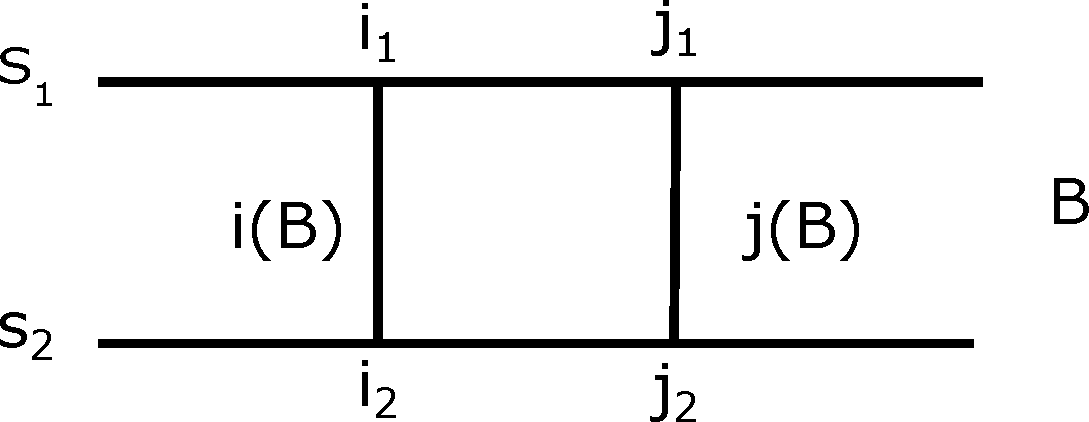
\includegraphics[width=0.6\linewidth]{block.pdf}
 		\centering
 		\caption{The block region $R(B)$ where the left and right most base pairs of $B$ concerning $S_1$}
 		\label{fig:block}
 	\end{figure}
 	
 	For a valid RRI, lets consider bases $k$ and $l$ form another allowed base pair. Then,
 	
 	\begin{center}
 		 $\forall_{B\in I } : \left(\nexists_{(k,l) \in P^1} : i(B)_1 \le k \le j(B)_1  \vee   i(B)_1 \le l \le j(B)_1 \right) $ \\$\wedge $\\ 	$\left(\nexists_{(k',l') \in P^1} : i(B)_2 \le k' \le j(B)_2  \vee  i(B)_2 \le l' \le j(B)_2\right) $
 	\end{center}
 	
 	where I is the union of all blocks (ie., all inter molecular base pairs)
 	We compute the joint structure between $S_1$ and $S_2$ through minimizing their total free energy. 
	
	\begin{figure}[tb]
		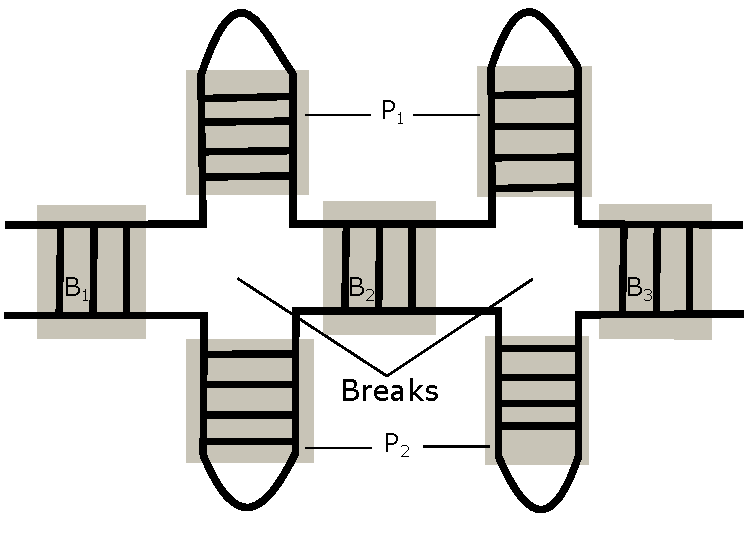
\includegraphics[width=0.5\linewidth]{break.pdf}
		\centering
		\caption{The interaction energy of RRI is the energy defined by the loops enclosed by all inter-molecular base pairs. $E(B_1)$ is the energy of block 1 and the $E(breaks)$ can be calculated from sum of all breaks.  }
		\label{fig:break}
	\end{figure}

		
	 The Energy for the block $E(B)$ can be calculated as  ,
	
	\begin{equation*}
	E(B) =  \sum_{\substack{i \in B \\ j \in B \\ \exists i < j}}E^{SBI}(i,j,k,l)
	\end{equation*}	
	
	where $j = argmin_{i' \in B \wedge i'>i}(i'_1)$. \\
	
		The $E(I)$ can be calculated as follows,
	
	\begin{center}
		$E(I) = E(  \uplus  B) + E_{init} $
	\end{center}
	\begin{center}
		where, $E(  \uplus  B) = \sum_B E(B) + E(breaks)$ and $E_{init}$ is fixed init score if $I$ $\neq$ $\phi$ 
	\end{center}

	In the fig ~\ref{fig:rnarna}, light violet colour represents the intramolecular loop with the intermolecular base pairs paired. We will need to find out, how to score them. Here, without further knowledge or energy parameters, we score it via standard loop scores ignoring the intermolecular pairings. The problem starts with the pseudoknot, in the loops where the positions are not paired within the loop ~\ref{fig:pseudoknot}.\\

	$E(breaks)$ is defined by the sum over all individual breaks between blocks (fig  ~\ref{fig:break} ). For the $E(breaks)$ it depends on the prediction model which is a tricky part and that will be discussed with the next section along with the approaches idea. Now, we will summarise the formal definition of energy of RRI. By using the above RRI equation, we can write overall energy of RRI as \\
	
	\begin{equation}
	\label{eq:rri}
	E(RRI) = E(P^1)+E(P^2)+E_{init}+ \sum_{B_i \in I}E(B_i) + \sum_{B_i \in I} E_{break} (B_i,B_{i+1}, P^1, P^2)
	\end{equation}
	
	
	\section{RNA-RNA Interaction Prediction Approaches}
	There are several available methods, that can be classified according to their underlying prediction strategies, each implicating unique capabilities and restrictions often not transparent to the non-expert user.\\ 
	Mostly for RNA-RNA interaction prediction methods are based on thermodynamic models and provide an efficient computation since Richard Bellman’s principle of optimality \citep{raden2018interactive} can be applied. RNA–RNA interaction prediction approaches are classified according to their algorithmic idea into hybrid-only interaction prediction,General interaction prediction, concatenation-based/cofolding interaction prediction , and accessibility-based interaction prediction. \\
	
	In the following subsections we will see about the approaches used for predicting the RNA-RNA interactions.\\

	
	\subsection{Hybrid}
	In hybrid-only interaction approach, the identification of RNA-RNA interaction doesn't consider intramolecular base pairs (fig ~\ref{fig:rnahybrid}) and they can be done with $O(nm)$ time and space complexity for two RNA sequences $S1$, $S2$ of lengths $n$ and $m$ respectively \citep{tjaden2006target}.\\
	
	\begin{figure}[H]
		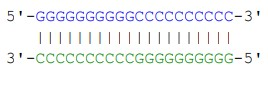
\includegraphics[width=0.4\linewidth]{rnahybrid}
		\centering
		\caption{ A full duplex structure where no intramolecular base pairs are assumed. The figure is taken from the paper \citep{wright2018structure}} 
		\label{fig:rnahybrid}
	\end{figure}
	
	
	 A dynamic programming approach using a simplified energy model with two dimensional table H is filled via the prefix-based recursion ~\ref{eq:2} for the nussinov like interaction prediction.\\
	 \begin{equation}
	 \label{eq:2}
	H_{ij} = max \begin{cases}
	H_{i-1,j-1}+1 & : \text{if $S^1_i$, $\overleftarrow{S^2_j}$ are compl. base pair }, \\
	H_{i-1,j} \\
	H_{i,j-1} ,
	\end{cases}
	\end{equation}
	Where $H_{ij}$ is the maximal number of intermolecular base pairs for the prefixes $S^1_1..i$	and $\overleftarrow{S^2_1..j}$ the reverse sequnce of $S^2$. The visual representation of the recursion scheme ~\ref{fig:hybrid} . The above equation is the s a variant of the global sequence alignment approach by \citep{needleman1970general} using scoring scheme i.e.,base pair instead of match/mismatch scoring for$S^1_i$, $\overleftarrow{S^2_j}$ no gap cost. Hence , when initialising $ H_{i,0} / H_{0,j} $ with 0, the $H_{n,m} $ gives the maximal number of intermolecular base pairs and we can trace back them. As stated above, this approach has very low runtime.\\
	
	 \begin{figure}[tb]
		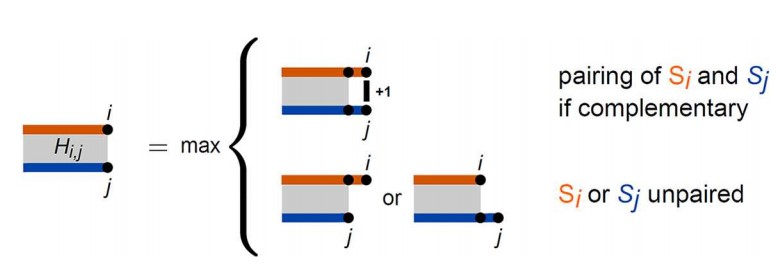
\includegraphics[width=0.8\linewidth]{hybrid}
		\centering
		\caption{Recursion scheme to maximize intermolecular base pairs between two RNAs $S1$ and $S2$ represented in orange/blue, respectively} 
		\label{fig:hybrid}
	\end{figure}

	In order to compute the energy of an RRI using equation ~\ref{eq:2} , no intra-molecular structure is considered, i.e. $P^1=P^2= \emptyset $ .
	
	Thus, eventually, only one block of inter-mol base pairs is modelled ie., $(I = B1)$ and no break is present. They are implemented in tools like TargetRNA, RNAhybrid, RNAplex. The main advantages of this approach is they allows temperature to taken into account, they are very fast and easy to calculate the significance of hits.  Since,  intramolecular base pairing is ignored they are used for the identification of short RNA's and overestimate the length of target sites. These disadvantages can be overcome by concatenation and accessibility based approaches.\\ 
	
	\subsection{General}
	One of the most common general approach that is used for predicting the two intermolecular RNA molecules is IRIS \citep{pervouchine2004iris} method. This method is basically implemented by dynamic programming where it is the product of the sequence alignment and two MFOLD type secondary structure prediction algorithms. They can predict \textit{general duplex structures}. This method is applied to some well known interactions such as OxyS with fhlA mRNA which basically forms a double kissing hairpin interactions as shown in below fig ~\ref{fig:doublekiss}.\\
	
	 \begin{figure}[tb]
		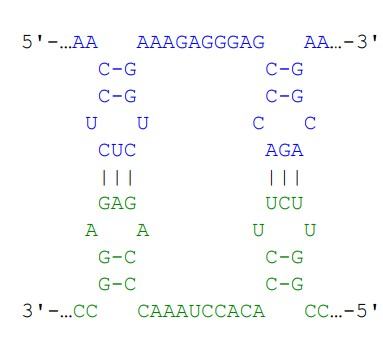
\includegraphics[width=0.4\linewidth]{doublekiss}
		\centering
		\caption{ Double kissing hairpin interaction. The blue and green denotes the first and second sequnence of RNA. Base pairs are denoted by dash. The picture is taken from the paper } 
		\citep{wright2018structure}
		\label{fig:doublekiss}
	\end{figure}
	
	It shares most common features with pseudoknots, but is less computationally intensive, secondary structure prediction system. The input is made up of two sequences of RNA. Each sequence can form its own nested secondary structure and hybridize into the other molecule. The computing time and space are $O(n^3m^3)$ and $O(n^2m^2)$ , where $n$ and $m$ are the length of the sequence sizes. The configuration of the oxyS-fhlA complex proposed in \citep{argaman2000fhla} consists of four neighboring stem loops, two in each of the molecules which connect, forming two stable kissing complexes. In this method, the main goal is the simulatinous optimization of intra and inter-molecular base pairing.\\

	\begin{figure}[tb]
		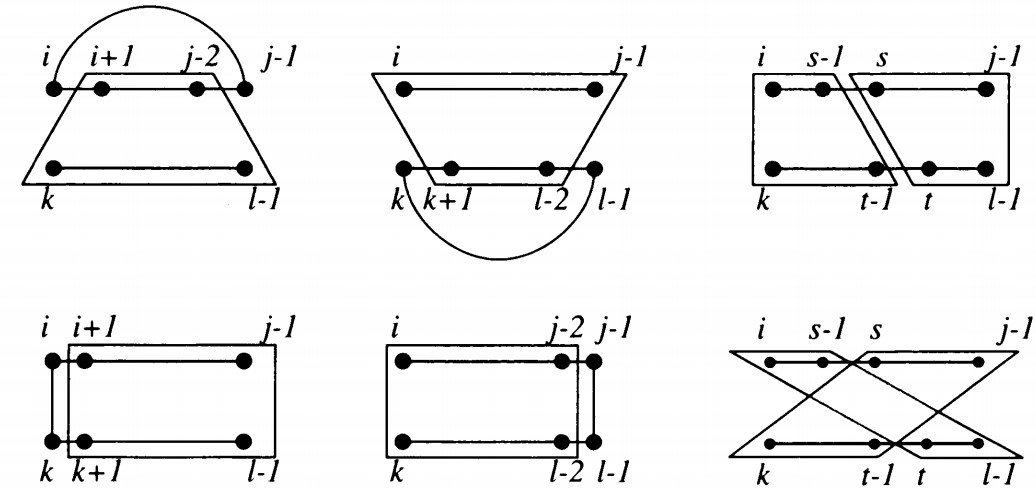
\includegraphics[width=0.9\linewidth]{iris}
		\centering
		\caption{ Depiction of the recursion $M^{i..k}_{j..l}$. Figure is taken from the paper} 
		\citep{pervouchine2004iris}
		\label{fig:iris}
	\end{figure}
	
	IRIS also supports crossing of consecutive blocks treated by the last recursion case in the lower right, which further complicates energy scoring of breaks. The energy contribution of general approach doesn't follow the interaction energy model instead they have pseudoknot energy. The energy associated with exterior pseudoknot can be given as \citep{xu2015physics} \\
	
		\begin{equation}
		G^{Pseudo} = \beta_1 + \beta_2 B^p + \beta_3 U^p
		\end{equation}
		
	where $\beta_1$ represents penalty for introducing a pseudoknot, $B^p$ is the number of base pairs that border the interior of the pseudoknot (i.e. number of paired positions), and $U^p$ is the number of unpaired bases inside the pseudoknot. reference to ~\ref{fig:pseudo} (right), here Bp=3 for the hairpin-PKs. If pseudoknot is inside a multiloop then they can be represented as $\beta_1^m$ ( by replacing the $\beta_1$) and if pseudoknot is inside another pseudoknot they can be  represented as $\beta_1^p$ (by replacing $\beta_1$).\\
	
	As an approximation, one could use E(PK-loop) such pseudoknot energy terms based on $G^Pseudo$ to score breaks. Note, to get an even more accurate overall energy scoring of an interaction, one would have to use pseudoknot energy terms also for such loops formed by intra-mol base pairs (refer ~\ref{fig:pseudo} (left)). for simplicity, formula (refer ~\ref{eq:2}) uses only nested energy terms to assess intra-molecular energies. Thus, the exact energy computation of the general approach is not covered by the formalizations used within this thesis.\\

	The time and space usage of IRIS are $ O(n^6)$ and $ O(n^4)$, respectively. The partition function version of RNA-RNA interaction prediction allows to predict the suboptimal interaction and its probabilities also the computation of probabilities of intermolecular interactions, which is used to access the stability. Due to its high complexity, several approaches for reducing the requirements of this method have been introduced.\\
	
	 
	\subsection{Concatenation}
	Concatenation or co-folding approach is used for predicting the interacting base pairs of two RNA molecules. Two or more sequences are concatenated  into a single sequence with special inter-spacing linker sequences. The final sequence is used within an adaptation of a standard structure prediction that takes  care of the linker sequences. The first implementation of this approach was by using Nearest neighbor model which was used for mfold and then implemented in tools like MutliRNAfold and RNAcofold.\\
	
	\begin{figure}[H]
		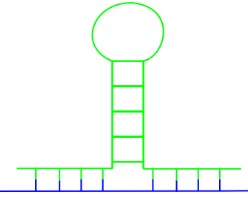
\includegraphics[width=0.3\linewidth]{concatenation}
		\centering
		\caption{ Green and blue are the two different RNA's that are interacting. } 
		\label{fig:concatenation}
	\end{figure}
	
	This is extension of single structure prediction recursion with a special handling of linker sequence. Here,the input is restricted to two RNA sequences that are concatenated by a linker of length $l+1$  to ensure the presence of a linker and that the concatenated sequence ends can form a base pair. We don't need any special energy treatment because the intra and inter molecular base pairs are treated equally.\\

	The energy for the concatenation approach, here the inter and intra molecular base pairs have same score and they are treated as a single sequence. Hence the breaks are considered as multi loop and scored accordingly. \\
		
	Concatentation-based approaches overcome the disadvantage of hybrid only approach by incorporating the competition of intra- and intermolecular base pairing. Still they cannot predict all the interaction patterns because  hybrid structures are nested. For example, interactions like kissing stem-loop or kissing hairpin-loop (as seen in fig ~\ref{fig:concat}) cannot be predicted because they form a pseduoknot by them. To predict these patterns we go for Accessibility based approaches.\\
	 \begin{figure}[tb]
		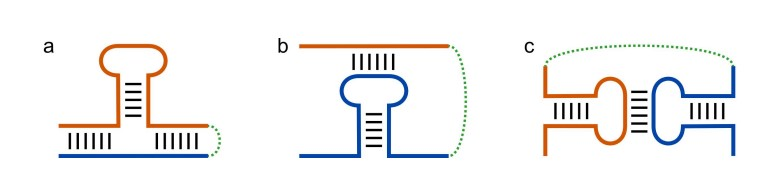
\includegraphics[width=0.9\linewidth]{concat}
		\centering
		\caption{a) Pattern that can be predicated by Concatenation b)Kissing stem-loop c) kissing hairpin interaction. The blue and orange are the two different RNA's and the dotted green is the linker , black lines represents the base pairs. } 
		\label{fig:concat}
	\end{figure}
	
	
	\subsection{Accessibility}
	Concatenation approaches cannot predict the structures which contains pseudoknots. To overcome the drawback of concatenation approach, Accessibility approaches has been introduced. The main aim of this approach is to ensemble properties of the single sequences that are necessary for the interaction.  It can predict single site an interaction pattern of two respective RNA subsequences. Tools like RNAup and IntaRNA can be used to predict such approaches. Here we have to neglect the intra molecular structure before the intermolecular interaction is formed. In order to form a stable interaction of intermolecular base pairs, the intra molecular base pairs has to be opened /broken. \\
	
	\begin{figure}[H]
		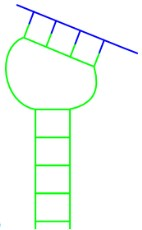
\includegraphics[width=0.2\linewidth]{acess}
		\centering
		\caption{ Green and blue are the two different RNA's that are interacting and forms pseudoknots. } 
		\label{fig:acess}
	\end{figure}

	We can classify single-site RNA-RNA interactions based on the structural context of the respective subsequences, which are\\
	
	\begin{itemize}
	\item exterior - not enclosed by any base pair.
	\item hairpin loop - directly enclosed by a base pair.
	\item non-hairpin loop - subsequence enclosed by two base pairs forming a bulge, interior or multi-loop.\\
    \end{itemize}
		
	IntaRNA can predict single-site interactions within any structural context of the respective subsequences, but concatenation-based approaches can only predict exterior-exterior context combinations. energy scoring differs from normal $E(RRI)$, since intra-mol structure only considered implicitly via ensemble energies.\\
	
	The term \textit{ensemble} refers to the set of all secondary structures which can be formed through an RNA sequence. In an RNA sequence S, the accessibility energy of a region[i, k ] is determined by the energy difference (referred to as ED):
	
	\begin{center}
		$ ED(i,k) = - (E^{all} - E_{i,k}^{u} )$\\
	\end{center}
	
	Where $E_{all}$ denotes the energy of the set of all possible secondary structures that can be generated by sequence S and $E_{i,k}^{u}$ denotes the energy of the ensemble of structures which have a single stranded area $ [i,k]$. \\
	The partition function is the total of all states Q over the Boltzmann factors. The energy of the ensemble $E^{all}$ is 
	
	\begin{center}
		
		$E^{all} = - RTln({Z_s})$
		
	\end{center}
	The probability of unpaired regions can be used for calculating the accessibility penalty for an interval $(i,k)$, as shown below: \\
	
	\begin{align*}
	ED(i,k) &= - (E(\mathcal{P}) - E(\mathcal{P}_{i,k}^{u}))\\
	&= E(\mathcal{P}_{i,k}^{u}) - (E(\mathcal{P}) \\
	&= - RTln({Z_s}_{i,k}^{u}) - - RTln({Z_s})\\
	&= - RTln(\frac{Z^u_{i_j}}{Z})\\
	&= - RTln(\mathcal{P}_{i,k}^{u})\\
	\end{align*}
	
	\begin{center}
	$ED^{1}_{i,k} = - RT \cdot \log(\mathcal{P}^{u1}_{i,k})$,\\ 
	$ED^{2}_{j,l} =  - RT \cdot \log(\mathcal{P}^{u2}_{j,l})$\\
	\end{center}

	
	Therefore, the alternative $E(RRI)$ formula :\\
	\begin{equation}
	E(RRI) = E(B1) + E_{init} + Eens(S1) + ED1 + Eens(S2) + ED2
	\end{equation} 
	
 	Since $ED = E^u - E ^{all}$ \\
	substituting $ED$ value in  $ED + E^{all}$ gives\\
	 $E^u - E ^{all}+ E^{all}$ \\
	 $ = E^{u}$\\
	 $E(RRI) = E(B1) + E_{init} + E^{u1} + E^{u2} $\\
		 
	The maximal number of base pairs $D^{i,k}_{j,l}$ for all interaction sites are computed using hybrid approach. Then the  unpaired probabilities $P^{u1}$ and $P^{u2}$ are tabularized for both sequences $S^1$ and $\overleftarrow{S^2}$, respectively using mcckaskill approach.\\
	
	\begin{figure}[tb]
		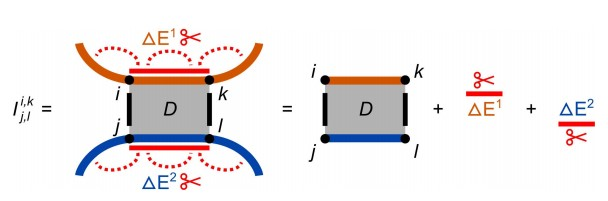
\includegraphics[width=0.9\linewidth]{access}
		\centering
		\caption{ Depiction how accessibility-based approaches score an interaction of two RNAs $S1$ and $S2$ in orange and blue respectively} 
		\label{fig:access}
	\end{figure}
	

	The energy of accessibility approach has no break , since the interaction I forms only one interaction block. Approaches like RNAup and IntaRNA use precalculated ED values for all possible interaction regions. They gives us how much energy is needed to free of intramolecular base pairs. \\
	
		\begin{figure}[tb]
		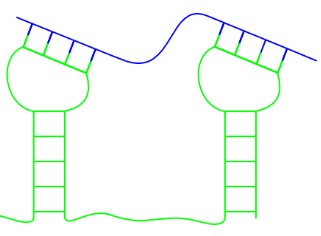
\includegraphics[width=0.4\linewidth]{doublestem}
		\centering
		\caption{ Double stem loop interaction cannot be handled by accessibility as they have two binding site.} 
		\label{fig:doublestem}
	\end{figure}
	
	
	The main drawback of accessibility approach is, it can handle only one non-crossing block. These approaches cannot be modelled correctly for the double kissing hairpin interaction which has more than one crossing blocks of interaction.\\
	
	
	\subsection{Comparison with approaches}
	In this subsection, we will see the comparison between the approaches for few interaction pattern. Below table ~\ref{table:1} gives the overview for which interaction pattern , the approaches can be used. \\
		\begin{table}[H]
				\caption{ Comparison of RNA-RNA interaction prediction approaches for different figures}
				\label{table:1}
		\begin{tabularx}{\textwidth}{ p{2cm}p{4.5cm}p{1.5cm}p{1cm}p{1cm}p{1cm}p{1cm}}
		\toprule
		\multicolumn{7}{c}{\textbf{Comparison of RRI approaches}}\\  
		\midrule
		\multicolumn{3}{c}{\textbf{RRI Pattern}}  & \multicolumn{4}{c}{\textbf{RRI prediction approaches}} \\
		\cmidrule(r){1-3}  \cmidrule(r){4-7}
		Figures & RRI description& No.of blocks& \rotatebox[origin=c]{90} {Hybrid}  &\rotatebox[origin=c]{90}{General}  &\rotatebox[origin=c]{90}{Concatenation}  &\rotatebox[origin=c]{90}{Accessibility} \\
		\hline
		\hline
		~\ref{fig:rnahybrid}&Full duplex structure&1 &yes &yes &yes &yes\\
		\hline
		~\ref{fig:concat} (a)& Nested joint structure without pseudoknots &2 & no &yes &yes &yes \\
		\hline
		~\ref{fig:concatenation}& Nested joint structure without pseudoknots &2 & no &yes &yes &yes \\
		\hline
		~\ref{fig:concat} (b)& Stem loop interaction &1 & no &yes &no &yes \\
		\hline
		~\ref{fig:acess} & Stem loop interaction &1 & no &yes &no &yes \\
		\hline
		~\ref{fig:concat} (c)& Kissing hairpin loop &1 & no &yes &no &yes \\
		\hline
		~\ref{fig:doublekiss}&Double kissing hairpin loop &2 &no &yes &no &no\\
		\hline
		~\ref{fig:rnarnainter}& Kissing stem interaction &2 &no &yes &no &no\\
		\hline
		~\ref{fig:doublestem}& Double kissing stem loop &2 &no &yes &no &no\\
		\hline
		
	\end{tabularx}
	\end{table}
	We could conclude that the accessibility based approach is the best approach for single site RNA-RNA interaction. As, they can't predict the multisite RRI because in IntaRNA model, we remove the base pairs while predicting, when they are no intramolecular base pairs are in between, it is considered to be a wrong model (ie., double kissing hairpin loop interaction).  To handle two or multi crossing blocks of interaction, we are introducing multisite accessibility based approach. The Multi-site RRI optimization is based on single-site IntaRNA predictions. Hence, we are going for the multisite accessibility based approach in the next chapter.\\

		
		
		
	\chapter{Multisite Accessibility Based  }
	
	In this chapter , we will see about the approach used for multisite interaction prediction for RNA. In simple words we could say, it is Multi-site RRI optimization based on single-site IntaRNA predictions. Accessibility-based RNA-RNA interaction prediction methods are typically modelling a single block of consecutive inter-molecular base pairs. Thus, interaction pattern that consists of multiple concurrently formed blocks can not be predicted. Within this thesis, we are developing and testing possibilities to efficiently predict concurrent blocks of interaction within an accessibility-based prediction model.The approach will be based on IntaRNA, which is one of the state-of-the-art programs for RNA-RNA interaction prediction.\\
	
	IntaRNA, developed by \citep{busch2008intarna} bioinformatics group at Freiburg University, is a general and fast approach to the prediction of RNA-RNA interactions incorporating both the accessibility of interacting sites as well as the existence of a user-definable seed interaction.  IntaRNA uses energy minimisation to find the best possible interaction.  \\
	
	Many RNAs interact via multiple synchronous, non-overlapping subinteractions (M-RRI), e.g. OxyS-fhlA. The simultaneous prediction of both intra- and inter-molecular base pairing allowing for multiple sites is computationally expensive. Some approaches in include IRIS, NUPACK, piRNA , etc., There are fast and reliable single interaction site (S-RRI) prediction tools like IntaRNA, that often show the additional sites within their suboptimal list, ie. are capable of modelling all sites individually but not in a joint prediction.	To overcome this, we use the iterative method in this thesis for finding the interaction between multiple blocks. \\
	
	\section{RNAup - Exact Recursion for single site}
	
	In the following, I will first introduce the RNAup-like exact recursions and then give an overview of IntaRNA heuristic version. IntaRNA is an interaction prediction tool developed for the prediction of mRNA target sites for small regulatory bacterial RNAs. The total energy score of the interaction is measured as the sum of the free hybridization energy and the free energy required to make the interaction sites available.\\
	
		\begin{figure}[tb]
		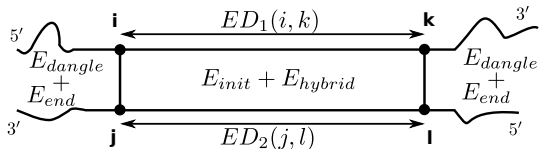
\includegraphics[width=0.6\linewidth]{inta}
		\centering
		\caption{ The energy contribution of IntaRNA. The image is taken from \citep{gelhausen2018constrained} } 
		\label{fig:inta}
	\end{figure}
	
	Scoring an interaction in IntaRNA is dependent on two energy contributions:\\
	
	\begin{itemize}
		\item \textbf{Hybridization energy} : energy value from intermolecular base pairings in the form of stackings, bulges or internal loops.  i.e., energy is a negative value. 
		\item \textbf{Accessibility energy} : An amount of energy needed to single-strand the interacting region, i.e. not include in intramolecular pairings. i.e., energy is a positive value. 
	\end{itemize}
	
	
	The energy of an ensemble of structures is calculated using a partition function \citep{mccaskill1990equilibrium} . Similarly, we get $ED(i,k)$ by calculating the partition function, ${Z_s}_{i,k}^{u}$ where $s_{i,k}^{u} $ is an ensemble of all structures which can be formed by a sequence S, with a single stranded region $[i,k]$. Refer to the section 1.4.4. Therefore,
	
		\begin{center}
		
		$ED(i,k) = - RTln({Z_s}_{i,k}^{u})$
		
	\end{center}
	


	\citep{muckstein2006thermodynamics} gives more detailed information on the same.
	The hybridization energy is measured using the Nearest Neighbor Energy Model. This represents the minimum free energy hybridization of two subsequences, where a base pair is generated by the leftmost positions of both subsequences.
	For sub-sequences $S_i^1...S_k^1$ and  $S_j^2...S_l^2$ , where $S^1$ is ordered from 5' to 3' and $S^2$ in the reverse order:

	
		\begin{center}
		
		$H(i,j,k,l) = min \{ E(P)$ | $(i, j) \in P \land (k,l) \in P \}$
		
	\end{center}
	
	The hybridization energy is calculated with a Zuker-like recursion.
	
	\begin{equation}
	H(i,j,k,l) = min \begin{cases}
	E_{init} \\
		\quad : \text{if $(S_i^1 , S_j^2 )$ can pair $i =k , j=l $}, \\	
	min_{r,s}\{ e^{SBI}(i,j,r,s)+ H(r,s,k,l)\} \\
	 \quad 	: \text{if $(S_i^1 , S_j^2 )$ and $(S_k^1 , S_l^2)$ can pair $i \neq k $ and $j \neq l $} ,\\
	\infty \\
	\quad : \text{otherwise},
	\end{cases}
	\end{equation}
	
	Here $e^{SBI} $ is the energy contribution of stack, bulge and internal loop. The traceback helps us to find the base pairs of optimal interaction with energy $H(i,j,k,l)$ . Both the accessibility and hybridisation energy forms the extended hybridisation energy which is the specific hybridisation between $S_i^1...S_k^1$ and  $S_j^2...S_l^2$ is given by, 
	
		\begin{equation}
	C(i,j,k,l) =  \begin{cases}
	H(i, j, k , l) + ED_1(i, k) + ED_2(j, l) \\
	\quad 	: \text{if $(S_i^1 , S_j^2 )$ and $(S_k^1 , S_l^2)$ can pair $i \neq k $ and $j \neq l $} ,\\
	\infty \\
	\quad : \text{otherwise},
	\end{cases}
	\end{equation}
	
	We get the time and space complexity of $O(n^2m^2)$ by limiting the loop size, which is still very high. When we limit the interaction length to l , it has a complexity of $O(nml^2)$ time and $O(nml^2)$ space. RNA molecules fold by intermolecular base pairing, by incorporating hydrogen bonds reduces free energy. Hence the system with the minimum free energy (mfe) is most likely the structure. The interaction with the minimum estimated free energy is probably the most stable structure and thus the structure fulfills the RNA molecule function.\\
	
	 \begin{equation*}
	mfe = \argmin_{i,j,k,l} C(i,j,k,l)
	\end{equation*}

	
	
	\section{IntaRNA -  Heuristic recursion for single site}
	
	The exact recursions are not suitable for the larger genome wide studies due to its high time and space complexity ie., $O(n^2m^2)$	where $n$ represents the length of query and $m$ is the length of target sequence. In order to overcome the time and space complexity problem, IntaRNA introduced the heuristic recursion. This recursion is based on sparsification technique where the matrix $c(i,j,k,l)$ many entries has same value and those values are not used often for the recursion. Hence, we consider only the right end of interaction $i, j$  which is single and locally optimal, instead of all the possible interaction. Similarly, we don't need to consider all possible ranges for time complexity. This will help us to reduce the space and time complexity to $O(nm)$. This is based on IntaRNA version 1 \& 2. The heuristic version is defined as:
	
	\begin{equation}
	C(i,j) =  \begin{cases}
	E_{init} + ED_1(i, i) + ED_2(j, j) \\
	\quad 	: \text{in the case of new interaction}\\
	min_{p,q}\{ e^{SBI}(i,j,p,q)+ C(p,q) - ED_1(p,K(p,q)) - ED_2(q,L(p,q))\\
	\quad \quad \quad \quad + ED_1(i,K(p,q)) + ED_2(j,L(p,q))\} \\
	\quad 	: \text{if $(S_i^1 , S_j^2 )$ can pair },\\
	\infty \\
	\quad : \text{otherwise},
	\end{cases}
	\end{equation}
	
	Here $K(p,q) , L(p,q)$ are the newly introduced matrices which are optimal. Since ED values are not additive, we have to subtract the old ED values before we add the new ED value.
	
	\section{Iterative scheme for multisite}
	 We use a Single-RRI prediction tool (namely IntaRNA) for the prediction of Multi-RRI. To this end, an iterative scheme is to be applied.
	
	 
	 \begin{itemize}
	 	 
	
	 \item Step 1: Firstly, we have to run IntaRNA and store minimum free energy as $B_1$ and the respective interaction site as $B_2$ which is empty.
	 \item Step 2: Then we get the 'blocking' constraint from step 1 by rerunning IntaRNA and predict conditional minimum free energy and site. Here we block $B_1$ (Constrainted IntaRNA) and we get $B_2'$ as minimum free energy. Then, the energy of an respective M-RRI can be computed from the two energies. ie., the energy of the conditional call can be added using the conditional probability.\\
	 \begin{center}
	 	 $E(B_1 \land B_2) = E(B_1) + E(B_2 | B_1)$ .
	 \end{center}
	 
	 \item Step 3: Since prediction (2) is conditional, the existence of the interaction from (2) can have effects on (1). Thus, one starts to iterate the procedure from (2) but fixes the conditional site. Then , we print the respective the $B_1$ and $B_2$. Finally, check for convergence: is the site from two-steps before retained $(B_2 == B'_2)$? If yes: convergence and stop iteration by printing the new $B_1 , B_2$. If no: repeat constraint prediction until convergence by swapping ( ie.,$B_2 = B_1; B_1 = B_2'$ ).
	 
	  \end{itemize}
  
  	
  	 \begin{figure}[tb]
  		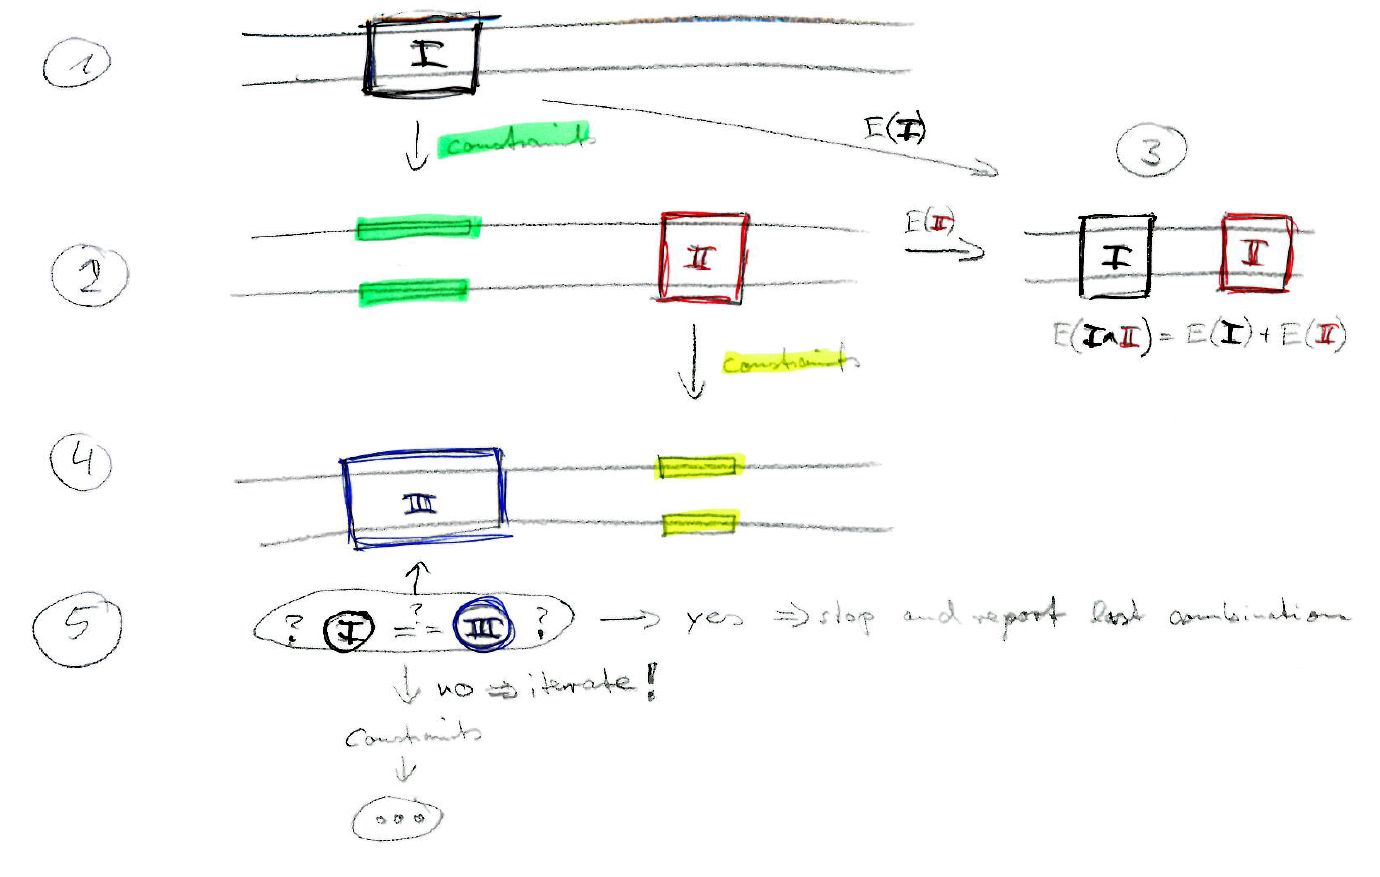
\includegraphics[width=0.9\linewidth]{idea}
  		\centering
  		\caption{ Iterative scheme that is used in this thesis.} 
  		\label{fig:idea}
 	 \end{figure}
  
  
  	Below is the flowchart representation for the same.\\
	
	% Define block styles
	\tikzstyle{decision} = [diamond, draw, fill=blue!20, 
	text width=4em, text badly centered, node distance=3cm, inner sep=0pt]
	\tikzstyle{block} = [rectangle, draw, fill=blue!20, 
	text width=5em, text centered, rounded corners]
	\tikzstyle{line} = [draw, very thick, color=black!50, -latex']
	\tikzstyle{cloud} = [draw, ellipse,fill=red!20,
	minimum height=2em]
	
	\begin{tikzpicture}[scale=2, node distance = 3cm, auto]
	% Place nodes
	\node [cloud, text width=2em] (start) {start};
	\node [block, right of=start , text width=4em] (store) {$B_1$ = mfe; $B_2$ = empty interaction site};
	\node [block, right of=store, node distance=3.3cm , text width=4em] (rerun) {$B_1$ = block; $B_2'$ = mfe};
	\node [decision, right of=rerun, node distance=3.3cm, text width=3em] (decide) {$B_2$ == $B_2'$};
	\node [block, below of=decide] (swap) {$B_2$ = $B_1$ ; $B_1$ = $B_2'$};
	\node [cloud, right of=decide] (stop) {stop};
	% Draw edges
	\path [line] (start) -- node[text width=1.2cm] {run IntaRNA} (store);
	\path [line] (store) -- node[text width=1.2cm] (run) {rerun IntaRNA}(rerun);
	\path [line] (rerun) -- node[text width=1.2cm] {print $B_1$ and $B_2$}(decide);
	\path [line] (decide) -- node [near start] {yes} (stop);
	\path [line] (decide) -- node {no}(swap);
	\path [line] (swap) -| (run);
	
	\end{tikzpicture}
	
	
	Below is the proof of why the energy of the conditional call can be just added. 
	
		\begin{align}	
	E(B_1 \land B_2) &= E(B_1) + E(B_2 | B_1) \nonumber\\	
	&= E_{hyb}(B_1 \land B_2) + ED(B_1 \land B_2) \nonumber\\	
	&= E_{hyb}(B_1)+E_{hyb}(B_2)-RTlog(\mathcal{P}^u(B_1 \land B_2)) \label{1}
	\end{align}

	 \begin{align}
	E(B_1) &= E_{hyb}(B_1) + ED(B_1)\nonumber\\
	&= E_{hyb}(B_1) - RTlog(\mathcal{P}^u(B_1)) \label{2}
	\end{align}
	
	\begin{align}
	E(B_2 | B_1) &= E_{hyb}( B_2 | B_1 )+ ED(B_2 | B_1)\nonumber \\
	& = E_{hyb}(B_2) - RTlog(\mathcal{P}^u(B_2 | B_1)) \label{3}
	\end{align}

Now, we add right end side values of Eqn ~\ref{3} + ~\ref{2}, we get,\\
	\begin{equation}
	\label{5}
	 E_{hyb}(B_1) + E_{hyb}(B_2) - RTlog(\mathcal{P}^u(B_1)) - RTlog(\mathcal{P}^u(B_2 | B_1))
	\end{equation}
	 
	As we know $log (A) + log (B) = log( A . B)$ , we apply this condition for log values in the Eqn~\ref{5}\\
	
	\begin{align*}
		-RTlog(\mathcal{P}^u(B_1)) - RTlog(\mathcal{P}^u(B_2 | B_1))\\
		-RTlog(\mathcal{P}^u(B_1) * \mathcal{P}^u(B_2 | B_1))\\
	\end{align*}
	
	Since $P(A \land B) = P(A) * P(B |A)$ we get,\\
	
	\begin{center}
		$-RTlog(\mathcal{P}^u(B_1 \land B_2))$
	\end{center}

 	After adding and simplifying the right end side values of Eqn ~\ref{3} + ~\ref{2} we get, \\
 	
 	\begin{equation}
 	\label{6}
 	E_{hyb}(B_1) + E_{hyb}(B_2) - RTlog(\mathcal{P}^u(B_1 \land B_2))\\
 	\end{equation}
	
	Now,  we see the equations ~\ref{6} and ~\ref{1} are equal ,\\
	\begin{equation}
	\label{7}
	E_{hyb}(B_1)+E_{hyb}(B_2)-RTlog(\mathcal{P}^u(B_1 \land B_2)) \Leftrightarrow E_{hyb}(B_1) + E_{hyb}(B_2) - RTlog(\mathcal{P}^u(B_1 \land B_2))
	\end{equation}
	
	We also know that \\
	\begin{align*}
		E_{hyb}(B_1) &= E_{hyb}(B_1)\\
		E_{hyb}( B_2 | B_1 ) &= \sum_{\forall loops in B_2}E_{hyb}(B_2)
	\end{align*}
	
	Hence proved. \\
	
	
	\chapter{Results}
	
	In order to evaluate the multi site interaction, I will compare the results of few RNA interactions with single site interaction tool "IntaRNA" . The multisite predictions gives you the total energy value of the interactions.\\ 
	
	
	\section{Setup}
	
	I have used the IntaRNA-3.1.3-windows-64bit version for my thesis. The following parameter has been set. The --outMode=C a flexible interface to generate RNA-RNA interaction output in CSV format (using ; as separator). The argument -n 1 or --outNumber=1 can be used to generate up to N interactions for each query-target pair. IntaRNA provides the possibility to constrain the accessibility computation using the --qAccConstr and --tAccConstr parameters. In this I have used "b" blocked by some other interaction (implies single-strandedness). The blocking of region is done for blocking the " B1" . For some applications it is needed to ignore dangling end energy contributions that reflect minor stabilizing (stacking) contributions of unpaired bases adjacent to a helix-closing base pair. They can be ignored via --energyNoDangles . It is possible to restrict the overall length an interaction is allowed to have. This can be done independently for the query and target sequence using --qIntLenMax and --tIntLenMax, respectively. We can alter indexing (independently for query and target) using the --qIdxPos0 and --tIdxPos0 parameters, respectively.\\
	
	\section{ Sample results}
	
	With the above setup , we were able to test few multi site RNA-RNA interactions.\\
	
%	\begin{table}[h]
%		\centering
%		\csvautotabular{datacollection.csv}
%		\caption{ Collections of multisite RNA interaction}
%	\end{table}
%	
	
		
	\begin{figure}
		\centering
		\begin{subfigure}{.5\textwidth}
			\centering
			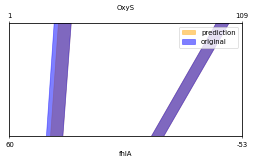
\includegraphics[width=.9\linewidth]{oxyleg}
			\caption{OxyS:fhlA}
			\label{fig:oxyleg}
		\end{subfigure}%
		\begin{subfigure}{.5\textwidth}
			\centering
			\includegraphics[width=.9\linewidth]{opp}
			\caption{oppA:Gcvb}
			\label{fig:opp}
		\end{subfigure}
		\begin{subfigure}{.5\textwidth}
			\centering
			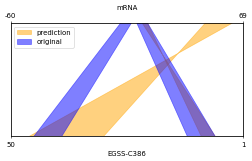
\includegraphics[width=.9\linewidth]{egsc386leg}
			\caption{mRNA:EGS S-C386}
			\label{fig:egsc386leg}
		\end{subfigure}%
		\begin{subfigure}{.5\textwidth}
			\centering
			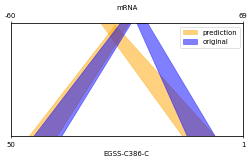
\includegraphics[width=.9\linewidth]{egsc386cleg}
			\caption{mRNA:EGS S-C386-C}
			\label{fig:egsc386cleg}
		\end{subfigure}
		\begin{subfigure}{.5\textwidth}
			\centering
			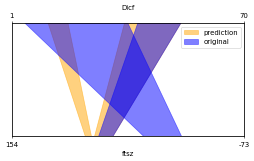
\includegraphics[width=.9\linewidth]{dicleg}
			\caption{Dicf:ftsz}
			\label{fig:dicleg}
		\end{subfigure}%
	\begin{subfigure}{.5\textwidth}
		\centering
		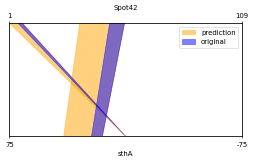
\includegraphics[width=.9\linewidth]{spoleg}
		\caption{spot42:stha}
		\label{fig:spotleg}
	\end{subfigure}
\begin{subfigure}{.5\textwidth}
	\centering
	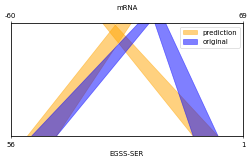
\includegraphics[width=.9\linewidth]{sserleg}
	\caption{mRNA:EGS S-SER}
	\label{fig:sserleg}
\end{subfigure}%
\begin{subfigure}{.5\textwidth}
	\centering
	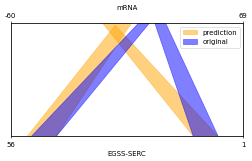
\includegraphics[width=.9\linewidth]{ssercleg}
	\caption{mRNA:EGS S-SERC}
	\label{fig:ssercleg}
\end{subfigure}%

		\caption{Multisite Interaction prediction for various RNA's}
		\label{fig:test}
			
	\end{figure}

\clearpage		
	\subsection{Oxys – fhla}
	
	OxyS interaction binds to a short sequence inside the fhlA mRNA coding region. This is one of the better site interaction examples where OxyS forms a stable kissing complex with fhlA. \\


	\begin{figure}[h!tb]
	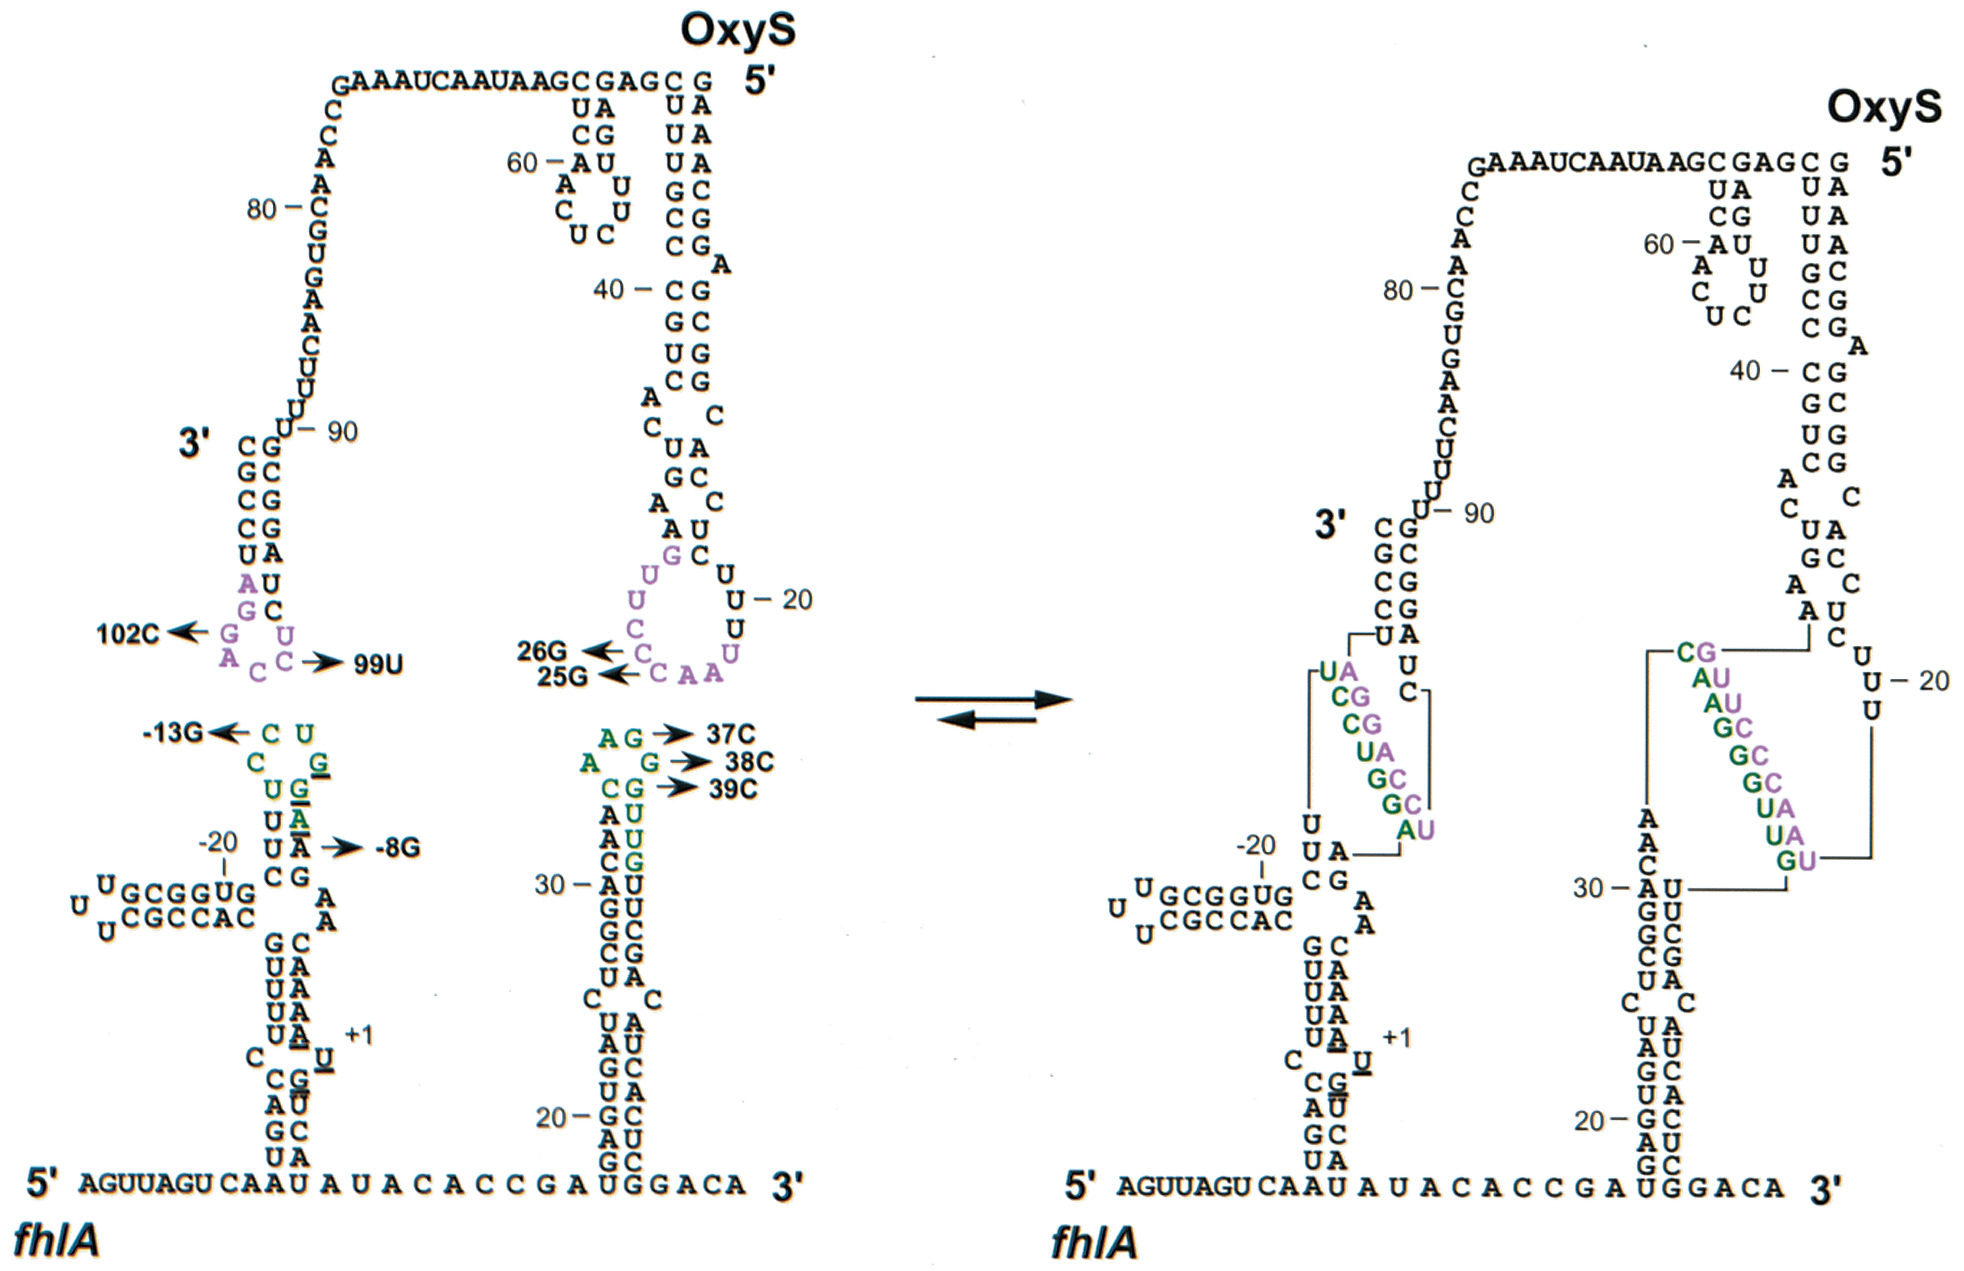
\includegraphics[width=1.0\linewidth]{oxys}
	\centering
	\caption{ Interaction of fhla-oxys } 
	\label{fig:oxys}
	\end{figure}

\begin{figure}[h!tb]
	\centering
	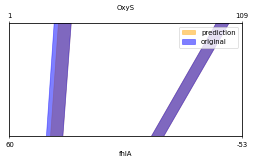
\includegraphics[width=.4\linewidth]{oxyleg}
	\caption{OxyS:fhlA}
	\label{fig:oxyleg}
\end{figure}

\clearpage
	
	
	
	\subsection{Spot42 – sthA }
	
	The Spot42 Interaction with sthA, Base-pairing RNA Spot 42 plays a large role in the suppression of catabolites in Escherichia coli by the direct suppression of genes involved in primary and secondary metabolism.\\
	
		\begin{figure}[h!tb]
		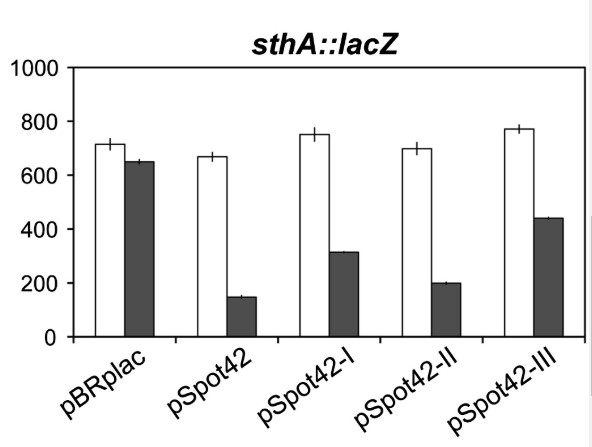
\includegraphics[width=0.6\linewidth]{spot42}
		\centering
		\caption{ Interaction of Spot42 – sthA } 
		\label{fig:spot42}
	\end{figure}

	\begin{figure}[h!tb]
		\centering
		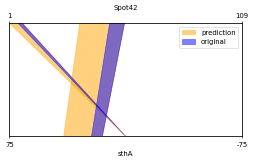
\includegraphics[width=.5\linewidth]{spoleg}
		\caption{spot42:stha}
		\label{fig:spotleg}
	\end{figure}

\clearpage

	\subsection{gcvB – oppA }
    The gcvB gene encodes two small, nontranslated RNAs that regulate OppA and DppA. The structure of the GcvB-oppA complex consists of two intermolecular helices that precede and follow the putative terminator. This is the example where there are four blocks are presented as per the {\citep{pervouchine2004iris}} . \\ 
	
		\begin{figure}[h!tb]
		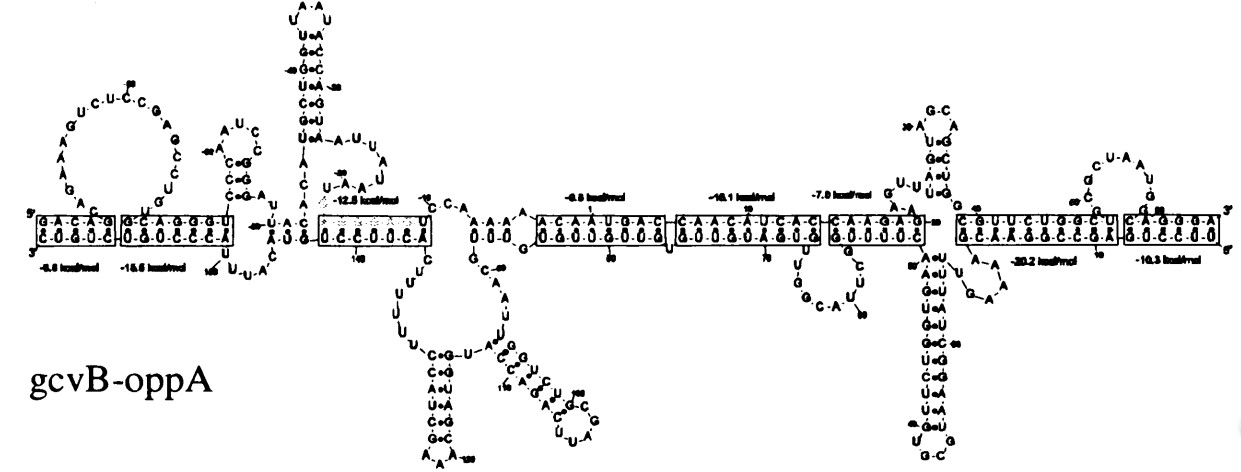
\includegraphics[width=1.0\linewidth]{oppa}
		\centering
		\caption{ Interaction of GCVB – oppA } 
		\label{fig:oppa}
	\end{figure}

	\begin{figure}[h!tb]
	\includegraphics[width=.5\linewidth]{opp}
	\centering
	\caption{ Interaction of GCVB – oppA } 
	\label{fig:opp}
\end{figure}


\clearpage
	
%	\item \textbf{GcvB – cycA }
%	
%	This interaction is an example for more than two site RNA interaction. In Escherichia coli, the GcvB gene encodes a small non-translated RNA that regulates several genes involved in transport of amino acids and peptides (including sstT, oppA and dppA). Microarray analysis identified cycA as an additional regulatory target of GcvB. In addition, deletion of the GcvB gene resulted in increased sensitivity to d-cycloserine, consistent with increased expression of cycA. The total energy for both the block is -23.19.
	
	\subsection{DicF - ftsZ }
	
	This is an example of a pseudknot (crossing interaction). We note that the dicF-ftsZ complex admits a area of complementarity, which gives rise to a generalized pseudo-knot. The composition of the dicF-ftsZ complex is identical to that of the dsrA-hns in which the dsrA RNA communicates with both the 5 'and 3' ends of the mRNA.\\   
	
		\begin{figure}[h!tb]
		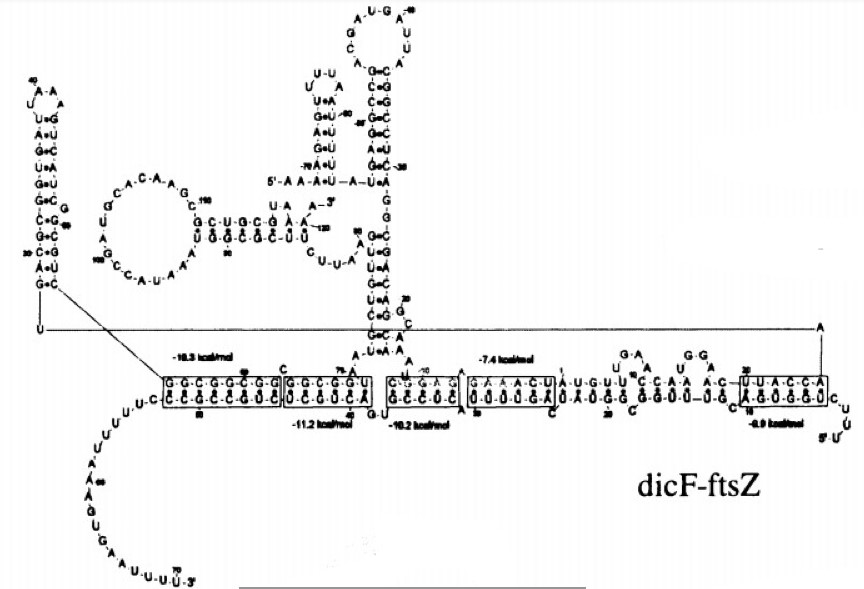
\includegraphics[width=1.0\linewidth]{dicf}
		\centering
		\caption{ Interaction of Dicf- ftsz } 
		\label{fig:dicf}
	\end{figure}

\begin{figure}[h!tb]
	\centering
	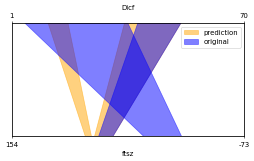
\includegraphics[width=.4\linewidth]{dicleg}
	\caption{Dicf:ftsz}
	\label{fig:dicleg}
\end{figure}

\clearpage
	\subsection{S-mRNA - EGS }
	
	 RNase P can be recruited to cleave any mRNA using a modified external reference sequence (EGS) that hybridizes with the target mRNAto shape a structure resembling the tRNA substrate. Just the exact sequence of the S mRNA around the targeting region is displayed (in red) and the EGS sequence is shown in blue. The RNase P cleavage site is labelled with an arrowhead. The sequences of S-SER and S-SER-C relative to T-stem and loop and the variable area of the tRNA molecule were derived from tRNASer, while those of S-C386 and S-C386-C were derived from the EGS variant C386.\\

	 
	 \begin{figure}[h!tb]
	 	\centering
	 	\begin{subfigure}{.25\textwidth}
	 		\centering
	 		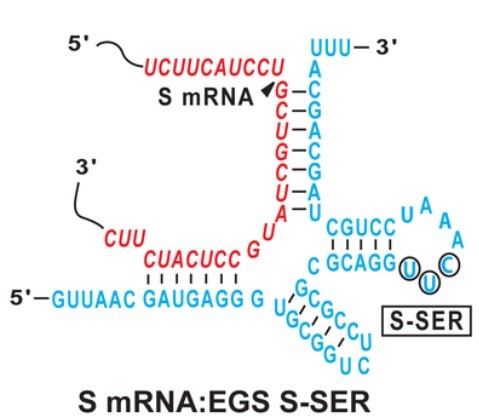
\includegraphics[width=.9\linewidth]{mrnaegs}	
	 		\label{fig:mrnaegs}
	 	\end{subfigure}

	 	\begin{subfigure}{.25\textwidth}
	 		\centering
	 		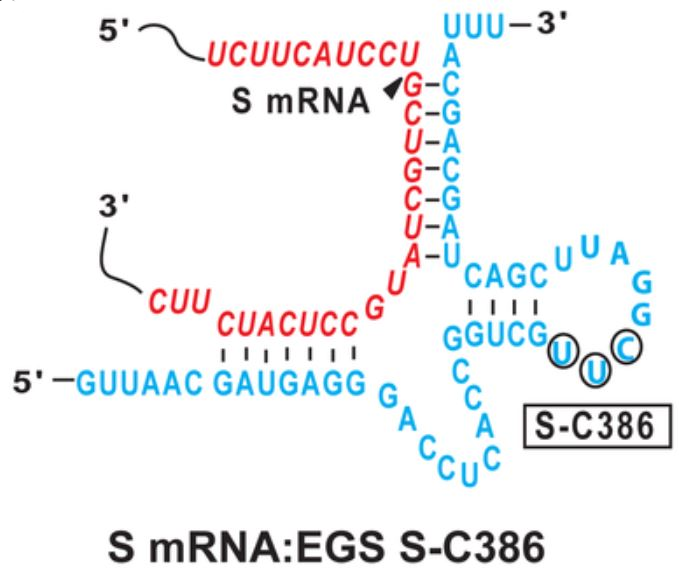
\includegraphics[width=.9\linewidth]{SC386}
	 		\label{fig:SC386}
	 	\end{subfigure}
	 	\begin{subfigure}{.25\textwidth}
	 		\centering
	 		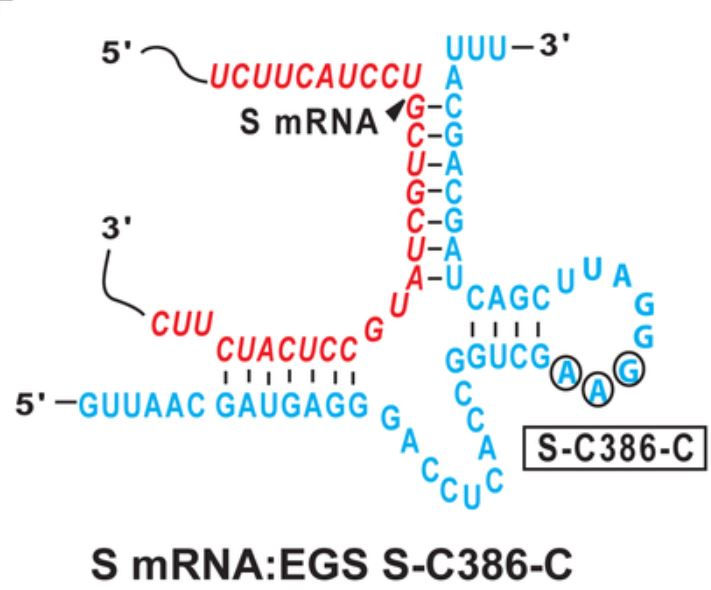
\includegraphics[width=.9\linewidth]{sc386c}
	 	
	 		\label{fig:sc386c}
	 	\end{subfigure}%
	 	\begin{subfigure}{.25\textwidth}
	 		\centering
	 		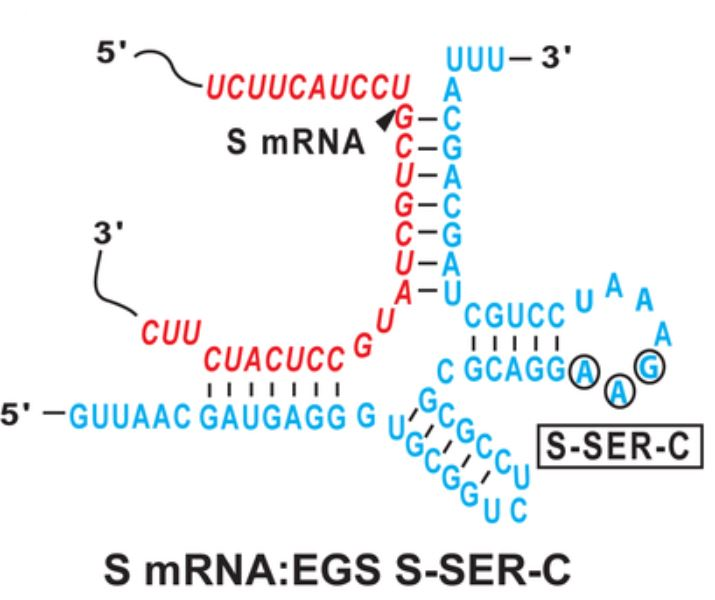
\includegraphics[width=.9\linewidth]{SERC}
	 		
	 		\label{fig:SERC}
	 	\end{subfigure}
 	\caption{An EGS resembling the structure of a tRNA.}
	 	\label{fig:test1}
	 \end{figure}
	 
	 \begin{figure}[h!tb]
	 	\centering
	 \begin{subfigure}{.5\textwidth}
	 	\centering
	 	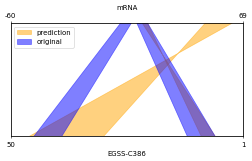
\includegraphics[width=.9\linewidth]{egsc386leg}
	 	\caption{mRNA:EGS S-C386}
	 	\label{fig:egsc386leg}
	 \end{subfigure}%
	 \begin{subfigure}{.5\textwidth}
	 	\centering
	 	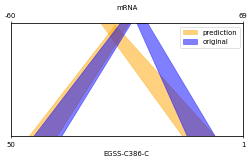
\includegraphics[width=.9\linewidth]{egsc386cleg}
	 	\caption{mRNA:EGS S-C386-C}
	 	\label{fig:egsc386cleg}
	 \end{subfigure}
 \end{figure}
\clearpage	


\subsection{Details of studied RRIs}

	
\begin{table}[H]
	
	\label{table:2}
	\begin{tabular}{ p{2cm}p{2.8cm}|p{2.8cm}p{1cm}p{1cm}|p{1cm}p{1cm}}
		\hline
		query:target& original& prediction& \rotatebox[origin=c]{90} {E(B1)}  &\rotatebox[origin=c]{90}{E(B1+B2)}  &\rotatebox[origin=c]{90}{1st index}  &\rotatebox[origin=c]{90}{length} \\
		\hline
		OxyS:fhlA&104:-15\&98:-9 30:34\&22:42
		&104:-15\&98:-9 30:34\&22:44&-4.37 &-7.99 &1:-53&109:113\\
		\hline
		Spot42:sthA&51:19\&49:21  7:NA\&5:NA & 55:15\&34:40 7:-8\&1:-2
		& -7.85 &-13.05 & 1:-75 &109:150 \\
		\hline
		oppA:Gcvb &-95:163\&-64:151 -17:142\&-11:136 -3:84\&19:49 39:18\&64:1  &67:14\&89:-9 152:63\&158:57
		& -14.57 &-26.38 & -95:3 &159:160\\
		\hline
		%			GcvB:cycA&  &161:175\&62:277 40:91\&34:97	& -18.88 &-23.19 & &201:300 \\
		%			\hline
		Dicf:ftsz&52:55\&39:69   \hbox{36:-12\&5:25}  &52:55\&35:73 12:82\&18:76	& -6.89 &-13.86 &1:-73 &70:227 \\
		\hline
		mRNA:EGSS-SER &26:7\&20:13 17:46\&11:52  &26:7\&20:11 & -10.3 &NA & 1:1 &29:56 \\
		\hline
		mRNA:EGSS-SER-C &26:7\&20:13 17:46\&11:52  &26:7\&20:11 & -10.28 &NA & 1:1 &29:56 \\
		\hline
		mRNA:EGS S-C386 &1:46\&7:40 10:13\&16:7 &
		47:48\&63:31 10:13\&16:7
		  & -8.15&-14.44 & -60:1 &129:50 \\
		\hline
		mRNA:EGS S-C386-C &1:46\&7:40 10:13\&16:7
		 &-1:47\&6:41 \hbox{-10:14\&-3:7}
		  & -8.14 &-13.24 & -60:1 &129:50 \\
		\hline
	\end{tabular}
	\caption{Collections of multisite RNA interaction }	
\end{table}


	
	\chapter{Discussion and conclusion}
	
	Here in the chapter we will discuss about the result section briefly.
	
	
	\section{OxyS – fhlA}
	 The first interaction is interaction between OxyS - fhlA. It is taken from the paper ~\cite{argaman2000fhla} .The pairing mechanism between the two RNAs is dramatically influenced by their structure. For this purpose, a full comprehension of the pairing process involves thorough knowledge of the individual RNA structures. \\
	 
	 OxyS binds wild-type fhlA mRNA shows that kissing complex forming between OxyS and fhlA results in a healthy anti-sense-target structure. The secondary structure of the 5 'end region of fhlA mRNA was predicted to include two stemloop structures. The findings of the study of the structure confirm the presence of the two structure. The result also show that the upper and lower portions of the Rbs stem- may be balanced by tertiary interactions.Awareness of the three-dimensional structure of the fhlA-OxyS kissing complex and the structural requirements that allow its development may have important consequences for the design of the artificial anti-sense RNAs. \\
	   
	 When tested , we find no difference in the Energy parameters and also with the hybridDB ( ie., hybrid in dot-bar notation). The total energy for both the block is -7.99. Here the sequence length for oxys starts from 1 to 109 and for fhla it is from -53 to 60. We use the parameter file for giving the target position to start from -53 ( indexing starts with 1 (tIdxPos0). We can clearly see from the ~\ref{fig:fhla} where the interaction that has been predicted and the original prediction from the same is almost same. \\
	 
	 \section{Spot42 – sthA }
	 This example is taken from \citep{beisel2011base} where Spot 42 secondary structure, previously re shown. Three consecutive nucleotides in each single-stranded region were mutated to block expected base-pair interactions with target mRNAs (I – III) refer ~\ref{fig:bei}. To validate base pairing through the three single-stranded regions of Spot 42, compensatory mutations have been made in the sthA. Such findings suggest that the base pairing with target mRNAs requires three single-stranded regions of Spot 42. The mutation in Region III influenced the repression of the fusion of sthA ( refer ~\ref{fig:bei1})  \\
	 

 \begin{figure}[h!tb]
	\centering
	\begin{subfigure}{.5\textwidth}
		\centering
		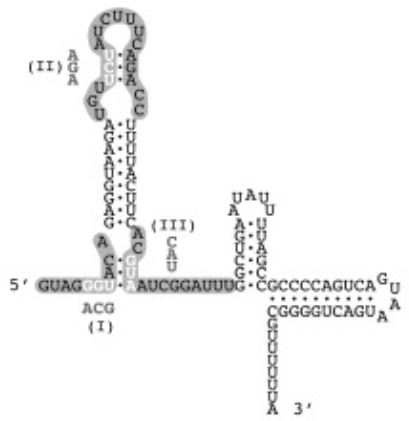
\includegraphics[width=.9\linewidth]{bei}
		\caption{Three single-stranded regions of spot42}
		\label{fig:bei}
	\end{subfigure}%
	\begin{subfigure}{.5\textwidth}
		\centering
		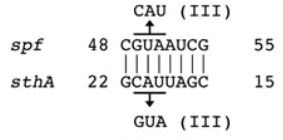
\includegraphics[width=.9\linewidth]{bei1}
		\caption{Mutation in Region III }
		\label{fig:bei1}
	\end{subfigure}
\end{figure}
	 
	 
	  Here when Spot42 interacts with sthA, we observed that the ED value changes. This is because , the unconstrained has been added to constrained value. Though there is no much difference in the total energy value, we are ignoring it. The total energy value is -26.38. In order to have the same ED values, we can use the --energyNoDangles option. Here for Spot42, we couldn't find the original interaction, hence we are comparing with the bar chart from the figure 2 from paper {\citep{beisel2011base}} . From the figure ~\ref{fig:spot42} we can clearly see . There is huge impact on pSpot32-III and pSpot32-I whereas less during the pSpot42-II. This is because, I and III are close in structure though they are far away from the sequence. We use the parameter file for giving the target position to start from -75.\\
	  
	  \section{gcvB – oppA }
	  The bulk of research investigating the modulation of gene expression in prokaryotes are aimed at explaining the influential roles that proteins perform in this function. Far less is understood regarding the functions of another type of molecules that have been shown to control gene expression: short, untranslated RNAs. OppA is the periplasmic-binding protein portion of the OppABCDF oligopeptide transport system. The functional consequence of deleting the gcvB gene is a derepression of the oppA. The mechanism of gcvB regulation of oppA is likely to be translational \citep{urbanowski2000gcvb}. In addition to their roles in the transport of dietary peptides, OppA have functions.\\
	  
	  Study of the gcvB sequence identified a complementarity area near the ribosome-binding sites of dppA and oppA mRNAs. The findings from {\citep{pulvermacher2008role}} indicate that various regions of GcvB have specific functions in the control of dppA and oppA mRNA. The Shine-Dalgarno sequence in the gcvB-oppA complex is obstructed, whereas the gcvB-oppA complex structure is located in the upstream region.This is very much in accordance with the assumption that the OppA Control seems to be at the translational stage, \\
	  
	As, we predict the multi block interaction, we have predicted the two sides of the interaction out of four. The total interaction energy for two sides of block is 26.88. For this example we used the parameter file and set the tIdxPos0=-95, 
	qIdxPos0=3 . \\
	
	 \section{DicF - ftsZ }
	 The function of dicF was predicted on the basis of the complementarity of DicF RNA with the ftsZmRNA binding region. DicF RNA is a 53-nucleotide gene formed in certain E.coli Mutants. Here, DicF RNA is an antisense regulator of ffsZ translation. A cell-division gene, ftsZ, was identified as the origin of dicF RNA by a genetic screen for suppressors of dicF-dependent inhibition of cell division ~\citep{tetart1992regulation}\\
	 
	 This example is taken from the paper \citep{pervouchine2004iris} .They say that dicF RNA has substantial complementarity with ftsZ mRNA in the area surrounding the ShineDalgarno sequence, which is compatible with the finding that dicF controls ftsZ through interaction with the ribosome binding. The dicF-ftsA relationship tends to be downstream of the start codon. As in the case of gcvB-dppA, it is proposed that dicF-mediated ftsA control occurs at mRNA level, whereas ftsA control occurs at translational level. Due to region of complementarity which leads to generalized pseudoknot  . \\
	 
	 For this example we used the parameter file and set the tIdxPos0=-73 , tIntLenMax=20 ( for restricting the overall length an interaction ).The total interaction energy for two sides of block that has been predicted by the tool is -13.86 \\
	 
	 \section{S-mRNA:EGS  }
	 
	 External guide sequences (EGSs) are RNA molecules that consist of a sequence that complements the target mRNA and recruits intracellular ribonuclease P (RNase P), a tRNA processing enzyme, for the precise degradation of the target mRNA. EGS  RNAs  derived  from  natural  tRNAsequences can be good in blocking gene expression in  bacteria. It is possible that an improvement in the RNase P cleavage rate could be attributed to additional tertiary interactions that theoretically stabilize the mRNA-EGS complex.\\
	 
	  The purpose of the research was to produce active EGS variants that could be used to attack mRNA, and to test variants to understand the process of how the EGS RNAs efficiently guide RNase P to the cleavage of the mRNA substrate. Variant C386 was chosen for this analysis because the EGS RNAsderived from this version are among the most efficient EGS's. EGS S-C386 was built by connecting the EGS domain of C386 to targeting sequences complementary to the S mRNA. The EGS, S-SER, originating from the normal tRNASer series, was also built. If this is the case, the binding affinity of the EGS variant (i.e. S-C386) to the target S RNA sequence might be greater than that of the EGS (i.e. S-SER) derived from the normal tRNA sequence. \\
	  
	  S-C386-C and S-SER-C were derived from S-C386 and S-SER, respectively, and incorporated simple substitutions (5'-UUC-3'- > AAG) at the three closely conserved locations in the T-loop of these EGSs.Nucleotides in these three positions are highly conserved among tRNA molecules and are essential for the folding and recognition of tRNA molecules by RNase P, so mutations in these positions are involved in the EGS process.S-C386-C and S-SER-C had the same anti-sense pattern to the targetS RNA series as S-C386 and S-SER ~\ref{fig:test1}  and had identical binding affinities to S38 as S-C386 and S-SER, respectively . S-C386-Cand S-SER-C can also be used as anti-sense regulation of such EGSs.\\
	 
	This example is taken from the paper \citep{zhang2013engineered }  .Here, the start of the S-mRNA is complementary to the end of the S-SER, which led to the crossing pattern. We can also clearly see that there is a shortage of the sequence. Also, the tails are not the actual , they are just the artificial one's. Due to its very short sequence , we took the 50nt long on the left side and right side of UCUUCAUCCUGCUGCUAUGCCUCAUCUUC of S-mRNA. The index position is taken from the site of cleavage .\\
	
	 Hence we add the parameterfile and set qIdxPos0=-10. We can also see that only one block is been predicted for the mRNA:EGS S-SER and mRNA:EGS S-SER-C. For the mRNA:EGS S-C386 and mRNA:EGS S-C386C two blocks are predicted. The total energy for mRNA:EGS S-C386 is -12.46 and mRNA:EGS S-C386C is -14.9  \\
	 
	
	\bibliographystyle{plainnat}
	\bibliography{ref}
	
\begin{appendices}

	\chapter{RNA Sequences}
	
	\begin{table}[H]
		
	\begin{tabular}{|p{1.5cm}|p{15cm}|}
		\hline
		RNA& Sequence\\
		\hline\hline	
		OxyS& GAAACGGAGCGGCACCTCTTTTAACCCTTGAAGTCACTGCCCGTTTCGAG AGTTTCTCAACTCGAATAACTAAAGCCAACGTGAACTTTTGCGGATCTCCAGGATCCGC \\
		\hline
		fhla&AGTTAGTCAATGACCTTTTGCACCGCTTTGCGGTGCTTTCCTGGAAGAACA AAATGTCATATACACCGATGAGTGATCTCGGACAACAAGGGTTGTTCGACATCACTCGGACA\\
		\hline
		spot42&GUAGGGUACAGAGGUAAGAUGUUCUAUCUUUCAGACCUUUUACUUCACGUAAUCG
		GAUUUGGCUGAAUAUUUUAGCCGCCCCAGUCAGUAAUGACUGGGGCGUUUUUUA\\
			\hline
		stha&GGGATCAATTGGCTTACCCGCGATAAAATGTTACCATTCTGTTGCTTTTATGTATAAGAA
		CAGGTAAGCCCTACCATGCCACATTCCTACGATTACGATGCCATAGTAATAGGTTCCGGCCCCGGCGGCGAAGG CGCTGCAATGGGCCTG\\
			\hline	
		GCVB &TTCCTGAGCCGGAACGAAAAGTTTTATCGGAATGCGTGTTCTGATGGGCTTTTGGCTT ACGGTTGTGATGTTGTGTTGTTGTGTTTGCAATTGGTCTGCGATTCAGACCACGGTAGCGAGACTACCCTTTT TCACTTCCTGTACATTTACCCTGTCTGTC\\
		\hline
		oppa& GACAGCAGAAAGUCUCCGAGCCUGUGCAGGGUCCCAAUCCGGGAUUACACAUGCUGG UUAAUACCAGUAAUUAUAAUGAGGGAGUCCAAAAAACAAUGACCAACAUCACCAAGAGAAGUUUAGUAGCAG CUGGCGUUCUGGCUGCGCUAAUGGCAGGGA\\
		\hline
		Dicf& TTTCTGGTGACGTTTGGCGGTATCAGTTTTACTCCGTGACTGCTCTGCCGCCCTTTTT AAAGTGAATTTT\\
		\hline
		ftsz& AAAAGAGTTTTAATTTTTATGAGGCCGACGATGATTACGGCCTCAGGCGACAGGCAC AAATCGGAGAGAAACTATGTTTGAACCAATGGAACTTACCAATGACGCGGTGATTAAAGTCATCGGCGTCGGCGGCGGCGGCGGTAATGCTGTTGAACACATGGTGCGCGAGCGCATTG AAGGTGTTGAATTCTTCGCGGTAAATACCGATGCACAAGCGCTGCGTAAAA\\	
			\hline
			egs& AACTTGTCCTGGTTATCGCTGGATGTGTCTGCGGCGTTTTATCATCTTCCTCTTCATCCTGCTGCTATGCCTCATCTTCTTGTTGGTTCTTCTGGACTATCAAGGTATGTTGCCCGTTTGTCCTCTAAT\\
			\hline
			S-SER& GTTAACGATGAGGGTGCGGTCTCCGCGCGCAGGTTCAAATCCTGCTAGCAGCATTT\\
			\hline
			S-SER-C&GTTAACGATGAGGGTGCGGTCTCCGCGCGCAGGAAGAAATCCTGCTAGCAGCATTT\\
			\hline
			S-C386&GTTAACGATGAGGGACCTCACCGGTCGTTCGGATTCGACTAGCAGCATTT\\
			\hline
			S-C386C& GTTAACGATGAGGGACCTCACCGGTCGAAGGGATTCGACTAGCAGCATTT\\
			\hline
	\end{tabular}
\caption{Table of RNAs with their corresponding sequence as used in this thesis.}
\end{table}

	
\end{appendices}
	
\end{document}